\documentclass[letterpaper,12pt,oneside]{article}\usepackage[]{graphicx}\usepackage[]{color}
%% maxwidth is the original width if it is less than linewidth
%% otherwise use linewidth (to make sure the graphics do not exceed the margin)
\makeatletter
\def\maxwidth{ %
  \ifdim\Gin@nat@width>\linewidth
    \linewidth
  \else
    \Gin@nat@width
  \fi
}
\makeatother

\definecolor{fgcolor}{rgb}{0.345, 0.345, 0.345}
\newcommand{\hlnum}[1]{\textcolor[rgb]{0.686,0.059,0.569}{#1}}%
\newcommand{\hlstr}[1]{\textcolor[rgb]{0.192,0.494,0.8}{#1}}%
\newcommand{\hlcom}[1]{\textcolor[rgb]{0.678,0.584,0.686}{\textit{#1}}}%
\newcommand{\hlopt}[1]{\textcolor[rgb]{0,0,0}{#1}}%
\newcommand{\hlstd}[1]{\textcolor[rgb]{0.345,0.345,0.345}{#1}}%
\newcommand{\hlkwa}[1]{\textcolor[rgb]{0.161,0.373,0.58}{\textbf{#1}}}%
\newcommand{\hlkwb}[1]{\textcolor[rgb]{0.69,0.353,0.396}{#1}}%
\newcommand{\hlkwc}[1]{\textcolor[rgb]{0.333,0.667,0.333}{#1}}%
\newcommand{\hlkwd}[1]{\textcolor[rgb]{0.737,0.353,0.396}{\textbf{#1}}}%

\usepackage{framed}
\makeatletter
\newenvironment{kframe}{%
 \def\at@end@of@kframe{}%
 \ifinner\ifhmode%
  \def\at@end@of@kframe{\end{minipage}}%
  \begin{minipage}{\columnwidth}%
 \fi\fi%
 \def\FrameCommand##1{\hskip\@totalleftmargin \hskip-\fboxsep
 \colorbox{shadecolor}{##1}\hskip-\fboxsep
     % There is no \\@totalrightmargin, so:
     \hskip-\linewidth \hskip-\@totalleftmargin \hskip\columnwidth}%
 \MakeFramed {\advance\hsize-\width
   \@totalleftmargin\z@ \linewidth\hsize
   \@setminipage}}%
 {\par\unskip\endMakeFramed%
 \at@end@of@kframe}
\makeatother

\definecolor{shadecolor}{rgb}{.97, .97, .97}
\definecolor{messagecolor}{rgb}{0, 0, 0}
\definecolor{warningcolor}{rgb}{1, 0, 1}
\definecolor{errorcolor}{rgb}{1, 0, 0}
\newenvironment{knitrout}{}{} % an empty environment to be redefined in TeX

\usepackage{alltt}
\usepackage[paperwidth=8.5in,paperheight=11in,top=1in,bottom=1in,left=1in,right=1in]{geometry}
\usepackage{setspace}
\usepackage[colorlinks=true,allcolors=Blue]{hyperref}
\usepackage[usenames,dvipsnames]{xcolor}
\usepackage{indentfirst}
\usepackage{titlesec}
\usepackage{multirow}
\usepackage{booktabs}
\usepackage{graphicx}
\usepackage{verbatim}
\usepackage{rotating}
\usepackage{tabularx}
\usepackage{outlines}
\usepackage{lineno}
\usepackage{array}
\usepackage{times}
\usepackage{cleveref}
\usepackage{acronym}
\usepackage[position=t]{subfig}
\usepackage{paralist}
\usepackage[noae]{Sweave}
\usepackage{natbib}
\usepackage{array}
\usepackage{pdflscape}
\usepackage{bm}
% \usepackage{showlabels}
\bibpunct{(}{)}{,}{a}{}{,}

% page margins and section title formatting
\linespread{1.5}
\setlength{\footskip}{0.5in}
\titleformat*{\section}{\Large\bf\em}
\titleformat*{\subsection}{\singlespace\large\bf}
\titleformat*{\subsubsection}{\singlespace\normalsize\bf\em}
\titlespacing{\section}{0in}{0in}{0in}
\titlespacing{\subsection}{0in}{0in}{0in}
\titlespacing{\subsubsection}{0in}{0in}{0in}

% cleveref options
\crefname{table}{Table}{Tables}
\crefname{figure}{Fig.}{Figs.}
\renewcommand{\figurename}{Fig.}

% aliased citations
\defcitealias{FLDEP12}{FLDEP 2012}
\defcitealias{HagyIR}{Hagy In review}
\defcitealias{USEPA06}{USEPA 2006}
\defcitealias{USEPA98}{USEPA 1998}

%acronyms
\acrodef{DEM}{Digital Elevation Model}
\acrodef{EPA}{Environmental Protection Agency}
\acrodef{doc}[$Z_c$]{depth of colonization}
\acrodef{GIS}{Geographic Information System}
\acrodef{IWR}{Impaired Waters Rule}
\acrodef{MSL}{mean sea level}
\acrodef{NAVD88}{North American Vertical Datum of 1988}
\acrodef{NOAA}{National Oceanic and Atmospheric Administration}

%knitr options


% get the version based on commit date


\IfFileExists{upquote.sty}{\usepackage{upquote}}{}
\begin{document}

\raggedbottom
\linenumbers
\raggedright
\urlstyle{same}
\setlength{\parindent}{0.5in}
\renewcommand\refname{References \vspace{12pt}}

\begin{singlespace}
\title{{\bf {\Large Quantifying seagrass light requirements using an algorithm to spatially resolve depth of colonization}}}
\author{
  {\bf {\normalsize Marcus W. Beck$^1$, James D. Hagy III$^2$, Chengfeng Le$^3$}}
  \\\\{\textit {\normalsize $^1$ORISE Research Participation Program}}
  \\{\textit {\normalsize USEPA National Health and Environmental Effects Research Laboratory}}
  \\{\textit {\normalsize Gulf Ecology Division, 1 Sabine Island Drive, Gulf Breeze, FL 32561}}
	\\{\textit {\normalsize Phone: 850-934-2480, Fax: 850-934-2401, Email: \href{mailto:beck.marcus@epa.gov}{beck.marcus@epa.gov}}}
  \\\\{\textit {\normalsize $^2$USEPA National Health and Environmental Effects Research Laboratory}}
	\\{\textit {\normalsize Gulf Ecology Division, 1 Sabine Island Drive, Gulf Breeze, FL 32561}}
	\\{\textit {\normalsize Phone: 850-934-2455, Fax: 850-934-2401, Email: \href{mailto:hagy.jim@epa.gov}{hagy.jim@epa.gov}}}
  \\\\{\textit {\normalsize $^3$ORISE Research Participation Program}}
  \\{\textit {\normalsize USEPA National Health and Environmental Effects Research Laboratory}}
  \\{\textit {\normalsize Gulf Ecology Division, 1 Sabine Island Drive, Gulf Breeze, FL 32561}}
  \\{\textit {\normalsize Phone: 850-934-9308, Fax: 850-934-2401, Email: \href{mailto:le.chengfeng@epa.gov}{le.chengfeng@epa.gov}}}
  \vspace{1in} 
  \\ Version Date:   Fri May 1 15:44:44 2015 -0500
	}
\date{}
\maketitle
\end{singlespace}
\clearpage

\section*{Abstract}



Physiological relationships between water clarity and growth of submersed aquatic vegetation have been used to  characterize nutrient limits in aquatic systems.  Specifially, the maximum \ac{doc} is a useful measure of seagrass growth that describes response to light attenuation in the water column.  However, lack of standardization among methods for estimating \ac{doc} has limited the description of habitat requirements at relevant spatial scales.  An algorithm is presented for estimating seagrass \ac{doc} using geospatial datasets that are commonly available for coastal regions.  A defining characteristic of the algorithm is the ability to estimate \ac{doc} using a flexible spatial unit such that the quantified values can be appplied to a specific area of interest.  These spatially-resolved estimates of \ac{doc} can then be related to light attenuation to develop a characterization of factors that limit seagrass growth, such as minimum light requirements at depth.  Four distinct coastal regions of Florida were evaluated to describe heterogeneity in seagrass growth patterns on relatively small spatial scales.  The analysis was extended to entire bay systems using \ac{doc} and satellite-derived light attenuation to quantify minimum light requirements on a broad scale using a systematic spatial context.  Sensitivity analyses indicated that confidence intervals for \ac{doc} were within reasonable limits for each case study, although the ability to quantify \ac{doc} varied with characteristics of the sampled data.  \ac{doc} estimates also varied along water quality gradients such that seagrass growth was more limited near locations with reduced water clarity. Site-specific characteristics that contributed to variation in growth patterns were easily distinguished using the algorithm as compared to more coarse estimates of \ac{doc}.  Minimum light requirements for the Indian River Lagoon (13.4\%) on the Atlantic Coast were substantially lower than those for Tampa Bay (30.4\%) and Choctawhatchee Bay (47.1\%) on the Gulf Coast.  High light requirements for the Gulf Coast may indicate regional differences in species requirements or additional factors, such as epiphyte growth, that further reduce light availability at the leaf surface.  A spatially robust characterization of seagrass \ac{doc} is possible for other regions because the algorithm is transferable with minimal effort to novel datasets.

\noindent \textit{Key words}: depth of colonization, estuary, Florida, light requirements, seagrasses, water clarity

\clearpage

\acresetall

\section{Introduction}

Seagrasses are ecologically valuable components of aquatic systems that have a critical role in shaping aquatic habitat.  These `ecosystem engineers' influence multiple characteristics of aquatic systems through interactions with many biological and abiotic components \citep{Jones94,Koch01}.  For example, seagrass beds create habitat for juvenile fish and invertebrates by reducing wave action and stabilizing sediment \citep{williams01,Hughes09}.  Seagrasses also respond to changes in water clarity through physiological linkages with light availability.  Seagrass communities in productive aquatic systems may be light-limited as increased nutrient loading reduces water clarity through increased algal concentration \citep{Duarte95}.  Empirical relationships between nutrient loading, water clarity, light requirements, and the maximum depth of seagrass colonization have been identified \citep{Duarte91,Kenworthy96,Choice14} and are often used to characterize light regimes sufficient to maintain seagrass habitat \citep{Steward05}.  Seagrass depth limits have also been used to establish quantititative targets for nutrient loading that will maintain water quality \citep{Janicki96}.  Seagrasses are integrative of conditions over time in relation to changes in nutrient regimes \citep{Duarte95} and are often preferred biological endpoints to describe ecosytem responses to perturbations relative to more variable taxa (e.g., phytoplankton).  Quantifying the relationship of seagrasses with water clarity is a useful approach to understanding ecological characteristics of aquatic systems with potential insights into system response to disturbance \citep{Greve05}.    

Many techniques have been developed for estimating seagrass depth limits to better understand water quality dynamics.  Such efforts have been useful for site-specific approaches where the analysis needs are driven by a particular question \citep[e.g.,][]{Iverson86,Hale04}. However, lack of standardization among methods has prevented broad-scale comparisons between regions and has even contributed to discrepancies between measures based on the technique used to measure depth of colonization \citep{Spears09}.  The availability of geospatial data that describe areal seagrass and bathymetric coverage suggests standardized techniques can be developed that could be applied across broad areas.  Conversely, site-specific approaches with such datasets typically quantify habitat requirements within predefined management units that may prevent generalizations outside of the study area. For example, \cite{Steward05} describe use of a segmentation scheme for the Indian River Lagoon to estimate seagrass depth limits for 19 distinct geospatial units.  Although useful for the specific study goals, substantial variation in growth patterns and water quality characteristics at different spatial scales may prevent more detailed analyses.  Methods for estimating seagrass depth limits should also be reproducible for broad-scale comparisons, while also maintaining flexibility based on the objectives. Such techniques can facilitate comparisons between regions given the spatial coverage and annual availability of many geospatial data sources.  

Estimating seagrass light requirements is a useful application of maximum depth limits and water clarity data.  Although growth of submersed aquatic plants is generally most limited by light availability \citep{Barko82,Hall90,Dennison93}, substantial variation in light requirements in the same community or between regions may suggest additional factors are limiting \citep{Dennison93,Choice14}.  Minimum light requirements for seagrasses are on average 11\% of surface irradiance \citep{Duarte91}, although values may range from less than 5\% to greater than 30\% depending on site conditions \citep{Dennison93}. Substantial variation in light requirements has been observed between species or based on regional differences in community attributes.  For example, significant variation in light requirements for the Gulf Coast of Florida were attributed to morphological and physiological differences between species and adaptations to regional light regimes \citep{Choice14}. Additional factors may also contribute to high estimates of light requirements, such as excessive epiphytic algal growth that reduces light availability on the leaf surface \citep{Kemp04}. Spatial heterogeneity in light requirements is, therefore, a useful diagnostic tool for identifying factors that affect seagrass growth. 

Water clarity data from satellite remote sensing products could be combined with depth of colonization estimates to develop a spatial description of seagrass light requirements.  Although algorithms have been developed for coastal waters to estimate surface reflectance from satellite data \citep{Woodruff99,Chen07}, this information has rarely been used to describe seagrass light requirements at a spatial resolution consistent with most remote sensing products.  Conversely, secchi observations can provide reliable measures of water clarity \citepalias{USEPA06}, although data can be biased by location and time.  Monitoring programs may have unbalanced coverage of aquatic resources with greater perceived importance relative to those that may have more ecological significance \citep{Wagner08,Lottig14}.  Morever, infrequent field measurements that are limited to discrete time periods are more descriptive of short-term variability rather than long-term trends in water clarity \citep{Elsdon09}.  Seagrasses growth patterns are integrative of seasonal and inter-annual patterns in water clarity, such that estimates of light requirements may be limited if water clarity measurements inadequately describe temporal variation.  Satellite remote sensing products can provide reliable estimates of water clarity and could be used to develop a more complete description of relevant ecosystem characteristics.  

Quantitative and flexible methods for estimating seagrass depth limits and light requirements can improve descriptions of aquatic habitat, thus enabling potentially novel insights into ecological characteristics of aquatic systems.  This article describes a method for estimating seagrass depth of colonization using geospatial datasets describing seagrass coverage and satellite remote sensing describing light attenuatuion of the water column to create a spatially-resolved and flexible measure.  An algorthm is described that estimates seagrass depth limits from coverage maps and bathymetric data using an \textit{a priori} defined area of influence. These estimates are combined with measures of water clarity to develop a spatial characterization of light requirements.  Study objectives are to\begin{inparaenum}[1\upshape)]
\item describe the method for estimating seagrass depth limits, 
\item apply the technique to four distinct regions of Florida to illustrate improved quantification of seagrass growth patterns with respect to depth, and
\item develop a spatial description of depth limits, water clarity, and light requirements for the case studies.  
\end{inparaenum}
The method is first illustrated using four relatively small areas of larger coastal regions followed by extension to entire estuaries to characterize spatial variation in light requirements, within and between regions.  Overall, these methods inform the description of seagrass growth patterns by developing a more spatially relevant characterization of aquatic habitat.  The method is applied to data from Florida, although the technique is easily transferable to other regions with coverage and water clarity data. 

\section{Methods}

\subsection{Study sites and data sources} \label{sec:data_srcs}

Four coastal locations in Florida were used as study sites: the Big Bend region (northeast Gulf Coast), Choctawhatchee Bay (panhandle), Tampa Bay (central Gulf Coast), and Indian River Lagoon (Atlantic coast) (\cref{tab:seg_summ,fig:seg_all}).  Sites were chosen to represent a regional distribution of coastal habitat in Florida, in addition to having available data and observed gradients in water quality. 

Coastal regions and estuaries in Florida are partitioned using a predefined segmentation scheme for developing numeric nutrient criteria.  These management segments were used for comparison to evaluate variation in growth patterns at different spatial scales.  For example, \Cref{fig:buff_ex1} shows variation in seagrass distribution for a management segment (thick polygon) in the Big Bend region of Florida.  The maximum depth colonization, as a red countour line, is based on a segment-wide estimate of all seagrasses within the polygon.  Although the estimate is not inaccurate, substantial variation in seagrass growth patterns at smaller spatial scales is not adequately described.  \ac{doc} is greatly over-estimated at the outflow of the Steinhatchee River (northeast portion of the segment) where high concentrations of dissolved organic matter reduce water clarity and naturally limit seagrass growth (personal communication, Nijole Wellendorf, Florida Department of Environmental Protection).  One segment within each region and smaller spatial units defined by the algorithm were first evaluated to illustrate use of the method.  Segments chosen for each region are shown in \cref{fig:seg_all}. A second analysis focused on quantifying seagrass depth limits for all of Choctawhatchee Bay, Tampa Bay, and the Indian River Lagoon to describe the spatial pattern of light requirements.

Geospatial data describing seagrass areal coverage combined with co-located bathymetric depth maps were used to estimate \ac{doc}.  These products are publically available in coastal regions of Florida through the US Geological Survey, Florida Department of Environmental Protection, Florida Fish and Wildlife Conservation Commission, and many watershed management districts.  Seagrass coverage maps were obtained for one chosen year in each of the study sites (\cref{tab:seg_summ}).  The original coverage maps were produced using photo-interpretations of aerial images to categorize seagrass as absent, discontinuous (patchy), or continuous.  We considered only present (continuous and patchy) and absent categories since differences between continuous and patchy coverage were often inconsistent between data sources. 

Bathymetric depth maps were obtained from the National Oceanic and Atmospheric Administration's (\acsu{NOAA}) National Geophysical Data Center (\url{http://www.ngdc.noaa.gov/}) as either \acp{DEM} or raw sounding data from hydroacoustic surveys.  Tampa Bay data provided by the Tampa Bay National Estuary Program are described in \citet{Tyler07}. Bathymetric data for the Indian River Lagoon were obtained from the St. John's Water Management District \citep{CPE97}.  The vertical datums varied such that \ac{NOAA} products were referenced to mean lower low water, Tampa Bay data were referenced to the \ac{NAVD88}, and the Indian River Lagoon data were referenced to mean sea level.  Prior to analysis, all bathymeric data were vertically adjusted to local \ac{MSL} using the \ac{NOAA} VDatum tool (\url{http://vdatum.noaa.gov/}) for comparability between data sources. Adjusted data were combined with seagrass coverage layers using standard union techniques for raster and vector layers in ArcMap 10.1 \citep{ESRI12}.  To reduce computation time, depth layers were first masked using a 1 km buffer of the seagrass coverage layer.  Raster bathymetric layers were converted to vector point layers to combine with seagrass coverage maps, described below.  

\subsection{Quantifying water clarity} \label{sec:clar_est}

Spatial variation in light requirements were explored using \ac{doc} and water clarity estimates for the entire areas of Choctawhatchee Bay, Tampa Bay, and the Indian River Lagoon. Limited clarity data in the Big Bend region prohibited analysis in this location.  Satellite images were used to create a gridded 1 km$^2$ map as estimated water clarity (m, Tampa Bay) or light extinction ($K_d$, m$^{-1}$, Choctawhatchee Bay).  Secchi data were used directly to evaluate light requirements for the Indian River Lagoon because satellite data were inestimable.

Daily MODIS (Aqua level-2) satellite data for the preceding five years from the seagrass coverage layer for Tampa and Choctawhatchee Bays were downloaded from the NASA website (\url{http://oceancolor.gsfc.nasa.gov/}). Images were reprocessed using the SeaWiFS Data Analysis System software (SeaDAS, Version 7.0). In Tampa Bay, water clarity was derived from daily MODIS images using a previously-developed algorithm \citep{Chen07}. Monthly and annual mean water clarity were calculated from the daily images and then averaged to create a single layer. Similarly, $K_d$ in Choctawhatchee bay was derived from MODIS using the QAA algorithm \citep{Lee05}.  Field measurements of $K_d$ for 2010 obtained at ten locations in Choctawhatchee Bay at monthly intervals were used to correct the unvalidated satellite $K_d$ values.  Specifially, annual mean field measurements of $K_d$ were compared to the annual mean satellite estimates in 2010.  An empirical correction equation was developed based on the difference between the cumulative distribution of the in situ $K_d$ estimates and the satellite estimated $K_d$ at the same locations.  The 2010 correction was applied to all five years of annual mean satellite data prior to averaging to create a single layer for further analysis.

Satellite estimates of water clarity were unobtainable in the Indian River Lagoon because of significant light scattering from bottom reflectance and limited resolution for narrow segments along the north-south axis.  Secchi data (meters, $Z_{secchi}$) within the previous ten years of the seagrass coverage data (i.e., 1999--2009) were obtained from update 40 of the \ac{IWR} database for all of the Indian River Lagoon.  More than five years of clarity data were used for Indian River Lagoon due to uneven temporal coverage.  Stations with less than five observations and observations that were flagged in the database indicating that the value was lower than the maximum depth of the observation point were removed.  Secchi data were also compared with bathymetric data to verify unflagged values were not missed by initial screening. 

\subsection{Estimating seagrass depth of colonization} \label{sec:est_method}

Seagrass \acl{doc} estimates used combined seagrass coverage maps and bathymetric depth data described above.  The combined layer was a point shapefile with attributes describing location (latitude, longitude), depth (m), and seagrass (present, absent).  Seagrass \ac{doc} values were estimated from these data by quantifying the proportion of points with seagrass at each observed depth.  Three unique measures obtained from these data are minimum ($Z_{c,\,min}$), median ($Z_{c,\,med}$), and maximum ($Z_{c,\,max}$) \acl{doc}.  Operationally, these terms describe characteristics of the seagrass coverage map with quantifiable significance. $Z_{c,\,max}$ is the deepest depth at which a significant coverage of mappable seagrasses occured independent of outliers, whereas  $Z_{c,\,med}$ is the median depth occurring at the deep water edge. $Z_{c,\,min}$ is the depth at which seagrass coverage begins to decline with increasing depth and may not be statistically distinguishable from zero depth, particularly in turbid waters.

The spatially-resolved approach for estimating \ac{doc} begins by choosing an explicit location in cartesian coordinates within the general boundaries of the available data.  Seagrass depth data (i.e., merged bathymetric and seagrass coverage data) that are located within a set radius from the chosen location are selected for estimating seagrass \ac{doc} values (sample areas in \cref{fig:buff_ex}). The estimate for each location is quantified from the proportion of sampled points that contain seagrass at decreasing 0.1 meter depth bins from the surface to the maximum depth in the sample (\cref{fig:est_ex1}).  Although the chosen radius for selecting data is problem-specific, the minimum radius should be large enough to sample a sufficient number of points for estimating \ac{doc}.  In general, a sufficient radius will produce a plot that indicates a decrease in the proportion of points that are occupied by seagrass with increasing depth. Plots with insufficient data may indicate a reduction of seagrass with depth has not occurred (e.g.,  nearshore areas) or seagrasses simply are not present.  If more than one location is used to estimate \ac{doc} (as in \cref{fig:buff_ex}), radii for each pointshould be chosen to reduce overlap with the seagrass depth data sampled by neighboring points.     

For each location, a curve is fit to the sampled depth points using non-linear regression to characterize the reduction in seagrass as a function of depth (\cref{fig:est_ex2}).  Specifically, a decreasing logistic growth curve is used with the assumption that seagrass decline with increasing depth is monotonic from the minimum depth of colonization followed by a gradual decline at the maximum depth.  The function is asymptotic at the minimum and maximum depths of colonization to constrain the estimates within the data domain. The curve is fit by minimizing the residual sums-of-squares with the Gauss-Newton algorithm \citep{Bates92} with starting parameters estimated from the observed data that are initial approximations of the curve characteristics.  The model has the following form:
\begin{equation} \label{eqn:prop}
 Proportion = \frac{\alpha}{1 + \mathrm{e}^{{\left(\beta - Z\right)/\gamma}}}
\end{equation}
where the proportion of points occupied by seagrass at each depth, $Z$, is defined by a logistic curve with an asymptote $\alpha$, a midpoint inflection $\beta$, and a scale parameter $\gamma$.  Finally, a simple linear curve is fit through the inflection point ($\beta$) of the logistic curve to estimate the three measures of depth of colonization (\cref{fig:est_ex3}).  The inflection point is considered the depth at which seagrass are decreasing at a maximum rate and is used as the slope of the linear curve.  The maximum depth of seagrass colonization, $Z_{c,\,max}$, is the x-axis intercept of the linear curve.  The minimum depth of seagrass growth, $Z_{c,\,min}$, is the location where the linear curve intercepts the upper asymptote of the logistic growth curve.  The median depth of seagrass colonization, $Z_{c,\,med}$, is the halfway between $Z_{c,\,min}$ and $Z_{c,\,max}$.  $Z_{c,\,med}$ is not always the inflection point of the logistic growth curve.

Estimates for each of the three \ac{doc} measures were obtained only if specific criteria were met.  These criteria were implemented as a safety measure that ensures a sufficient amount and appropriate quality of data were sampled within the chosen radius.  First, estimates were provided only if a sufficient number of seagrass depth points were present in the sampled data to estimate a logistic growth curve.  This criteria applies to the sample size as well as the number of points with seagrass in the sample.  Second, estimates were provided only if an inflection point was present on the logistic curve within the range of the sampled depth data.  This criteria applied under two scenarios where the curve was estimated but a trend was not adequately described by the sampled data.  That is, estimates were unavailable if the logistic curve described only the initial decrease in points occupied as a function of depth.  The opposite scenario occurred when a curve was estimated but only the deeper locations beyond the inflection point were present in the sample.  Third, the estimate for $Z_{c,\,min}$ was set to zero depth if the linear curve through the inflection point intercepted the upper asymptote of the logistic curve at x-axis values less than zero.  The estimate for $Z_{c,\,med}$ was also shifted to the depth value halfway between $Z_{c,\,min}$ and $Z_{c,\,max}$ if $Z_{c,\,min}$ was fixed at zero.  Finally, estimates were considered invalid if the 95\% confidence interval for $Z_{c,\,max}$ included zero.  In such cases, the three measures are not statistically distinguishable, although a useful estimate for $Z_{c,\max}$ is provided.  Methods to determine confidence bounds are described below.  

\subsection{Estimating uncertainty}

Confidence intervals for the \ac{doc} values were estimated using a Monte Carlo simulation approach that used the variance-covariance matrix of the logistic model parameters \citep{Hilborn97}.  Confidence intervals were constructed by repeated sampling of a multivariate normal distribution to evaluate the uncertainty in the inflection point in \cref{eqn:prop}.  The sampling distribution assumes:
\begin{equation}
x \sim N(\mu, \Sigma)
\end{equation}
\noindent where $x$ is a predictor variable used in \cref{eqn:prop} (depth) that follows a multivariate normal distribution with mean $\mu$, and variance-covariance matrix $\Sigma$.  The mean values are set at the depth value corresponding to the inflection point on the logistic curve from the observed model, whereas $\Sigma$ is the variance-covariance matrix of the model parameters ($\alpha$, $\beta$, $\gamma$).  A large number of samples ($n = 10000$) were drawn from the distribution to characterize the uncertainty of the depth value of the inflection point.  The 2.5\textsuperscript{th} and 97.5\textsuperscript{th} percentiles of the sample were considered bounds on the 95\% confidence interval.  This approach was used because uncertainty from the logistic curve is directly related to uncertainty in each of the \ac{doc} estimates that are based on the linear curve through the inflection point. Upper and lower limits for each \ac{doc} estimate were obtained by fitting new linear curves through the upper and lower limits of the initial depth value. (i.e., \cref{fig:est_ex3}).

Nonlinear least squares models were based on the \texttt{nls} and \texttt{SSlogis} functions that used a self-starting logistic growth model \citep{Bates92,RDCT14}.  Multivariate normal distributions were simulated using functions in the MASS package \citep{Venables02}.  Geospatial data were imported and processed using functions in the rgeos and sp packages \citep{Bivand08,Bivand14}.  

\subsection{Evaluation of spatial heterogeneity of seagrass depth limits}

Spatially-resolved estimates of \ac{doc} were obtained for several locations in each of the four segments described above (\cref{fig:seg_all}).  A regular grid of locations for estimating each of the three \ac{doc} values was created for each segment.  Spacing between sample points was 0.01 decimal degrees ($\approx$1 km at 30 degrees N latitude) and the sampling radius for each location was set to 0.02 decimal degrees.  The sample radius allowed complete utilization of the seagrass data while minimizing overlap.  Finally, a single segment-wide estimate using all data at each study site was used for comparisons.  Departures from the segment-wide estimate at finer scales were considered evidence of spatial heterogeneity in seagrass growth and improved clarity of description as a result.  

\subsection{Relating depth of colonization and water clarity}

Relationships between seagrass depth limits and water clarity were explored by estimating light requirements for the entire areas of Choctawhatchee Bay, Tampa Bay, and Indian River Lagoon.  Seagrass depth limits that were co-located with estimates of water clarity, either as satellite-based estimates or in situ secchi observations, were related using empirical light attenuation equations.  The Lambert-Beer equation describes the exponential decrease of light availability with depth:
\begin{equation} \label{eqn:lambeer}
I_{z} = I_{O} \cdot \exp\left(-K_{d} \cdot Z\right)
\end{equation}
\noindent such that the irradiance of incident light at depth $Z$ ($I_{Z}$) can be estimated from the irradiance at the surface ($I_{O}$) and a light extinction coefficient ($K_{d}$). Light requirements of seagrass can be estimated by rearranging \cref{eqn:lambeer}:
\begin{equation} \label{eqn:perclight}
\% \ light = \exp\left(-K_{d} \cdot Z_{c,\,max}\right)
\end{equation}
\noindent where the percent light requirements are a function of the estimated $Z_{c,\,max}$ and light extinction. If $K_d$ estimates are unavailable, a conversion factor can be used to estimate the light extinction coefficient from secchi depth $Z_{secchi}$, such that $c = K_{d} \cdot Z_{secchi}$, where $c$ has been estimated as 1.7 \citep{Poole29,Idso74}:
\begin{equation} \label{eqn:cperclight}
\% \ light = \exp\left(-\left(\frac{1.7}{Z_{secchi}}\right)\cdot Z_{c,\,max}\right)
\end{equation}

Two approaches were used to estimate light requirements based on the availability of satellite data or in situ water clarity (see \label{sec:clar_est}).  For locations with satellite data (Choctawhatchee and Tampa Bay), a regular grid of sampling points was created as before to estimate $Z_{c,\,max}$ and sample the continuous layer of satellite-derived water clarity.  Grid spacing was different in each bay (0.005 for Choctawhatchee Bay, 0.01 for Tampa Bay) to account for variation in spatial scales of seagrass coverage.  \Cref{eqn:perclight} was used to estimate light requirements at each point for Choctawhatchee Bay and \cref{eqn:cperclight} was used for Tampa Bay.  Similarly, the geographic coordinates for each in situ secchi measurement in the Indian River Lagoon were used as locations for estimating $Z_{c,\,max}$ and light requirements using \cref{eqn:cperclight}.  Excessively small estimates for light requirements were removed for Indian River Lagoon which were likely caused by shallow secchi observations that were not screened during initial data processing.  A critical difference between the satellite and secchi data was that a more complete spatial description of light requirements was possible in the former case due to continuous coverage, whereas descriptions using secchi data were confined to the original sampling locations.  Sampling radii for locations in each bay were chosen to maximize the number of points with estimable values for $Z_{c,\,max}$ (as described in \cref{sec:est_method}), while limiting the upper radius to adequately describe variation in seagrass growth patterns for emphasizing gradients in light requirements. Radii were fixed at 0.04 decimal degrees for Choctawhatchee Bay, 0.1 decimal degrees for Tampa Bay, and 0.15 decimal degrees for Indian River Lagoon.

\section{Results}

\subsection{Segment characteristics and seagrass depth estimates}

% data for inline expressions


Each coastal region varied by several characteristics that potentially explain variation of seagrass growth (\cref{tab:seg_summ}).  Mean surface area was 191.2 square kilometers, with area decreasing for the Big Bend (271.4 km), Upper Indian River Lagoon (228.5 km), Old Tampa Bay (205.5 km), and Choctawhatchee Bay (59.4 km) segments.  Mean depth was less than 5 meters for each segment, excluding Western Choctawhatchee Bay which was slightly deeper than the other segments (5.3 m).  Maximum depths were considerably deeper for Choctawhatchee Bay (11.9 m) and Old Tampa Bay (10.4 m), as compared to the Big Bend (3.6 m) and Indian River Lagoon (1.4 m) segments. Seagrasses covered a majority of the surface area for the Big Bend segment (74.8 \%), whereas coverage was much less for Upper Indian River Lagoon (32.8 \%), Old Tampa Bay (11.9 \%), and Western Choctawhatchee Bay (5.9 \%).  Visual examination of the seagrass coverage maps for the respective year of each segment indicated that seagrasses were not uniformly distributed (\cref{fig:seg_all}).  Seagrasses in Western Choctawhatchee Bay were sparse with the exception of a large patch located to the west of the inlet connection with the Gulf of Mexico.  Seagrasses in the Big Bend segment were located throughout with noticeable declines near the outflow of the Steinhatchee River, whereas seagrasses in Old Tampa Bay and Upper Indian River Lagoon were generally confined to shallow areas near the shore. Seagrass coverage showed a partial decline toward the northern ends of both Old Tampa Bay and Upper Indian River Lagoon segments.  Water clarity as indicated by average secchi depths was similar between the segments (1.5 m), although Choctawhatchee Bay had a slightly higher average (2.1 m).     

% seagrass estimates from table


The segment-wide estimates of \ac{doc} indicated that seagrasses generally did not grow deeper than three meters in any of the segments (\cref{tab:est_summ}).  Maximum and median depth of colonization were deepest for the Big Bend segment (3.7 and 2.5 m, respectively) and shallowest for Old Tampa Bay (1.1 and 0.9 m), whereas the minimum depth of colonization was deepest for Western Choctawhatchee Bay (1.8 m) and shallowest for Old Tampa Bay (0.6 m).  In most cases, the averages of all grid-based estimates were less than the whole segment estimates, indicating a left-skewed distribution of estimates at finer spatial scales.  For example, the average of all grid estimates for $Z_{c,\,max}$ in the Big Bend region indicated seagrasses grew to approximately 2.1 m, which was 1.6 m less than the whole segment estimate.  Although reductions were not as severe for the average grid estimates for the remaining segments, considerable within-segment variation was observed depending on grid location.  For example, the deepest estimate for $Z_{c,\,min}$ (2 m) in the Upper Indian River Lagoon exceeded the average of all grid locations for $Z_{c,\,max}$ (1.7 m).  $Z_{c,\,min}$ also had minimum values of zero meters for the Big Bend and Old Tampa Bay segments, suggesting that seagrasses declined continously from the surface for several locations.   

Visual interpretations of the grid estimates provided further information on the distribution of seagrasses in each segment (\cref{fig:all_ests}).  Spatial heterogeneity in depth limits was particularly apparent for the Big Bend and Upper Indian River Lagoon segments.  As expected, depth estimates indicated that seagrasses grew deeper at locations far from the outflow of the Steinhatchee River in the Big Bend segment.  Similarly, seagrasses were limited to shallower depths at the north end of the Upper Indian River Lagoon segment near the Merrit Island National Wildlife Refuge. Seagrasses were estimated to grow at maximum depths up to 2.2 m on the eastern portion of the Upper Indian River Lagoon segment.  Spatial heterogeneity was less distinct for the remaining segments although some patterns were apparent.  Seagrasses in Old Tampa Bay grew slightly deeper in the northeast portion of the segment and declined to shallower depths near the inflow at the northern edge.  Spatial variation in Western Choctawhatchee Bay was minimal, although the maximum \ac{doc} estimate was observed in the northeast portion of the segment.  As expected, \ac{doc} values could not be estimated where seagrasses were sparse or absent, nor where seagrasses were present but the sampled points did not show a decline with depth.  The former scenario was most common in Old Tampa Bay and Western Choctawhatchee Bay where seagrasses were unevenly distributed or confined to shallow areas near the shore.  The latter scenario was most common in the Big Bend segment where seagrasses were abundant but locations near the shore were inestimable given that seagrasses did not decline appreciably within the depths that were sampled.   


Uncertainty in $Z_{c,\,max}$ indicated that confidence intervals were generally acceptable (i.e., greater than zero), although the ability to discriminate between the three depth estimates varied by segment (\cref{fig:all_ests,tab:sens_summ}). Uncertainty for all estimates as the average width of the 95\% confidence intervals for all segments was 0.2 m.  Greater uncertainty was observed for Western Choctawhatchee Bay (mean width was 0.5 m) and Old Tampa Bay (0.4 m), compared to the Big Bend (0.1 m) and Upper Indian River Lagoon (0.1 m) segments.  The largest confidence interval for each segment was 1.4 m for Old Tampa Bay, 1.6 m for Western Choctawhatchee Bay, 0.5 m for the Big Bend, and 0.8 m for the Upper Indian River Lagoon segments.  Most confidence intervals for the remaining grid locations were much smaller than the maximum in each segment (e.g., an extreme central location of the Upper Indian River Lagoon, \cref{fig:all_ests}).  A comparison of overlapping confidence intervals for $Z_{c,\,min}$, $Z_{c,\,med}$, and $Z_{c,\,max}$ at each grid location indicated that not every measure was unique.  Specifically, only 11.1\% of grid points in Choctawhatchee Bay and 28.2\% in Old Tampa Bay had significantly different estimates, whereas 82.4\% of grid points in the Indian River Lagoon and 96.2\% of grid points in the Big Bend segments had estimates that were significantly different.  By contrast, all grid estimates in Choctawhatchee Bay and Indian River Lagoon had $Z_{c,\,max}$ estimates that were significantly greater than zero, whereas all but 12.4\% of grid points in Old Tampa Bay and 8\% of grid points in the Big Bend segment had $Z_{c,\,max}$ estimates significantly greater than zero. 

\subsection{Evaluation of seagrass light requirements}

Estimates of water clarity, seagrass depth limits, and corresponding light requirements for all locations in Choctawhatchee Bay, Tampa Bay, and the Indian River Lagoon indicated substantial variation, both between and within the different bays.  Satellite-derived estimates of light attenuation for Choctawhatchee Bay (as $K_d$, \cref{fig:kd_choc}) and Tampa Bay (as clarity, \cref{fig:clarity_tb}) indicated variation between years and along major longitudinal and lateral axes.  For Choctawhatchee Bay, $K_d$ estimates for western and central segments were substantially smaller than those for the more shallow, eastern segment.  Maximum $K_d$ values were also observed in earlier years (e.g., 2003, 2004).  Clarity estimates for Tampa Bay also showed an increase towards more seaward segments, with particularly higher clarity along the mainstem.  Clarity in 2006 was relatively lower than other years, with noticeable increases in 2007 and 2008.  In situ secchi observations for the Indian River Lagoon followed a clear latitudinal gradient with higher values in more southern segments (\cref{fig:light_irl}).  Very few measurements were available for the Upper Indian River Lagoon and Banana River segments, likely due to water clarity exceeding the maximum depth in shallow areas.



Seagrass \ac{doc} estimates were obtained for 259 locations in Choctawhatchee Bay, 566 locations in Tampa Bay, and 37 locations in the Indian River Lagoon (\Cref{tab:light_summ,fig:light_choc,fig:light_tb,fig:light_irl}).  Mean $Z_{c,\,max}$ for each bay was 2.5, 1.7, and 1.3 m for Choctawhatchee Bay, Tampa Bay, and Indian River Lagoon, respectively, with all values being significantly different between bays (ANOVA, $F=$ 326.9, $df =$ 2, 859, $p < 0.001$, followed by Tukey multiple comparison, $p<0.001$ for all).  Generally, spatial variation in $Z_{c,\,max}$ followed variation in light requirements for broad spatial scales with more seaward segments or areas near inlets having lower light requirements.  Mean light requirements were significantly different between all bays (ANOVA, $F=$ 463.7, $df =$ 2, 859, $p < 0.001$, Tukey $p<0.001$ for all), with a mean requirement of 47.1\% for Choctawhatchee Bay, 30.4\% for Tampa Bay, and 13.4\% for Indian River Lagoon.  Significant differences in light requirements between segments within each bay were also observed (ANOVA, $F =$ 12.1, $df =$ 2, 256, $p < 0.001$ for Choctawhatchee Bay, $F =$ 84.6, $df =$ 3, 562, $p < 0.001$ for Tampa Bay, $F =$ 7.6, $df =$ 6, 30, $p < 0.001$ for Indian River Lagoon).  Post-hoc evaluation of all pair-wise comparisons of mean light requirements between segments within each bay indicated that significant differences were apparent for several locations.  Significant differences were observed between all segments in Choctawhatchee Bay ($p<0.001$ for all), except the central and western segments (\cref{fig:light_choc}).  Similarly, significant differences in Tampa Bay were observed between all segments ($p<0.05$ for all), except Middle Tampa Bay and Old Tampa Bay (\cref{fig:light_tb}).  Finally, for the Indian River Lagoon, significant differences were observed only between the Lower Central Indian River Lagoon and the Upper ($p<0.001$) and Lower Mosquito Lagoons ($p = $ 0.023),  the Lower Indian River Lagoon and the Upper ($p<0.001$) and Lower Mosquito Lagoons ($p =$ 0.013), and the Upper Central Indian River and the Upper Mosquito Lagoon ($p = $0.018) (\cref{fig:light_irl}).  Small sample sizes likely reduced the ability to distinguish between segments in the Indian River Lagoon.

\section{Discussion}

Seagrass depth of colonization is tightly coupled to variation in water quality such that an accurate method for estimating $Z_{c,\,max}$ provides a biologically-relevant description of aquatic habitat.  Accordingly, the ability to estimate seagrass depth of colonization and associated light requirements from relatively inexpensive sources of information has great value for developing an understanding of potentially limiting factors that affect ecosystem condition.  To these ends, this study presented an approach for estimating seagrass depth of colonization from existing geospatial datasets that has the potential to greatly improve clarity of description within multiple spatial contexts.  We evaluated four distinct coastal regions of Florida to illustrate utility of the method for describing seagrass depth limits at relatively small spatial scales and extended the analysis to entire bay systems by combining estimates with water clarity to characterize spatial variation in light requirements.  The results indicated that substantial variation in seagrass depth limits were observed, even within relatively small areas of interest.  Estimated light requirements also indicated substantial heterogeneity within and between entire bays, suggesting uneven distribution of factors that limit seagrass growth patterns.  To our knowledge, such an approach has yet to be implemented in widespread descriptions of aquatic habitat and there is great potential to expand the method beyond the current case studies.  The reproducible nature of the algorithm also enables a context-dependent approach given the high level of flexibility.

\subsection{Evaluation of the algorithm}

The algorithm for estimating seagrass depth of colonization has three primary advantages that facilitated a description of aquatic habitat in each of the case studies.  First, the application of non-linear least squares regression provided an empirical means to characterize the reduction of seagrass coverage with increasing depth.  This approach was necessary for estimating each of the three depth limits ($Z_{c,\,min}$, $Z_{c,\,med}$, $Z_{c,\,max}$) using the maximum slope of the curve.  The maximum rate of decline describes a direct and estimable physiological response of seagrass to decreasing light availability such that each measure provided an operational characterization of growth patterns (see \cref{sec:est_method}).  The regression approach also allowed an estimation of confidence in \ac{doc} values by accounting for uncertainty in each of the three parameters of the logistic growth curve ($\alpha$, $\beta$, $\gamma$). Indications of uncertainty are required components of any esimation technique that provide a direct evaluation of the quality of data used to determine he model fit.  By default, estimates with confidence intervals for $Z_{c,\,max}$ that included zero were discarded to remove highly imprecise estimates.  Despite this restriction, some examples had exceptionally large confidence intervals relative to neighboring estimates (e.g., center of Upper Indian River Lagoon, \cref{fig:all_ests}), which suggests not all locations are suitable for applying the algorithm. The ability to estimate \ac{doc} and to discriminate between the three measures depended on several factors, the most important being the extent to which the sampled seagrass points described a true reduction of seagrass coverage with depth.  Sampling method (e.g., chosen radius) as well as site-specific characteristics (e.g., bottom-slope, actual occurrence of seagrass) are critical factors that directly influence confidence in \ac{doc} estimates.  A pragmatic approach should be used when applying the algorithm to novel data such that the location and chosen sample radius should be defined by the limits of the analysis objectives. 

A second advantage is that the algorithm is highly flexible depending on the desired spatial context.  Although this attribute directly affects confidence intervals, the ability to choose a sampling radius based on a problem of interest can greatly improve the description of aquatic habitat given site-level characteristics.  The previous example described for the Big Bend region highlights this flexibility, such that a segment-wide estimate was inadequate for characterizing $Z_{c,\,max}$ that was limited near the outflow of the Steinhatchee river.  The ability to choose a smaller sampling radius more appropriate for the location indicated that $Z_{c,\,max}$ reflected known differences in water clarity near the outflow relative to other locations in the segment.  However, an important point is that a segment-wide estimate is not necesarily biased such that a sampling radius that covers a broad spatial area could be appropriate depending on the analysis needs.  If the effect of water clarity near the outflow was not a concern, the segment-wide estimate could describe seagrass growth patterns for the larger area without inducing descriptive bias.  However, water quality standards as employed by management agencies are commonly based on predefined management units, which may not be appropriate for all locations.  The flexibility of the algorithm could facilitate the development of point-based standards that eliminate the need to develop or use a pre-defined classification scheme.  In essence, the relevant management area can be defined a priori based on known site characteristics.

The ability to use existing geospatial datasets is a third advantage of the algorithm.  Further, bathymetry data and seagrass coverage are the only requirements for describing $Z_c$ in a spatial context.  These datasets are routinely collected by agencies at annual or semi-annual cycles for numerous coastal regions.  Accordingly, data availability and the relatively simple method for estimating \ac{doc} suggests that spatial descriptions could be developed for much larger regions with minimal effort.  The availability of satellite-based products with resolutions appropriate for the scale of assessment could also facilitate a broader understanding of seagrass light requirements when combined with \ac{doc} estimates.  However, data quality is always a relevant issue when using secondary information as a means of decision-making or addressing specific research questions.  Methods for acquiring bathymetric or seagrass coverage data are generally similar between agencies such that the validity of comparisons from multiple sources is typically not a concern.  However, one point of concern is the minimum mapping unit for each coverage layer, which is limited by the resolution of the original aerial photos and the comparability of photo-interpreted products created by different analysts.  Seagrass maps routinely classify coverage as absent, patchy, or continuous.  Discrepancies between the latter two categories between regions limited the analysis to a simple binary categorization of seagrass as present or absent. An additional evaluation of comparability between categories for different coverage maps could improve the descriptive capabilities of \ac{doc} estimates.

\subsection{Heterogeneity in growth patterns and light requirements}

Variation in $Z_c$ for each of the case studies, as individual segments and whole bays, was typically most pronounced along mainstem axes of each estuary or as distance from an inlet.  Greater depth of colonization was observed near seaward locations and was also most limited near river inflows.  Although an obvious conclusion would be that depth of colonization is correlated with bottom depth, i.e., seagrasses grow deeper because they can, a more biologically-relevant conclusion is that seagrass depth of colonization follows expected spatial variation in water clarity.  Shallow areas within an estuary are often near river outflows where discharge is characterized by high sediment or nutrient loads that contribute to light scattering and increased attenuation.  Variation in \ac{doc} along mainstem axes was not unexpected, although the ability to characterize within-segment variation for each of the case studies was greatly improved from more coarse estimates.  Seagrasses may also be limited in shallow areas by tidal stress such that a minimum depth can be defined that describes the upper limit related to dessication stress from exposure at low tide.  Coastal regions of Florida, particularly the Gulf Coast, are microtidal with amplitudes not exceeding 0.5 meters.  Accordingly, the effects of tidal stress on limiting the minimum depth of colonization were not apparent for many locations in the case studies such that $Z_{c,\,min}$ estimates were often observed at zero depth.  Although this measure operationally defines the depth at which seagrasses begin to decline with decreasing light availability, $Z_{c,\,min}$ could also be used to describe the presence or absence of tidal stress.

The use of light attenuation data, either as satellite-derived estimates or in situ secchi observations, combined with \ac{doc} estimates provided detailed and previously unavailable characterizations of light requirements within the three estuaries.  Requirements were lowest for the Indian River Lagoon, whereas estimates were higher for Tampa Bay and highest for Choctawhatchee Bay. Requirements for the Indian River Lagoon were generally in agreement with other Atlantic coastal systems \citep{Dennison93,Kemp04}, such that requirements typically did not exceed 25\% with mean requirements for whole bay estimated at 13.4\%.  However, light requirements for Indian River Lagoon were based on secchi observations with uneven spatial and temporal coverage, which potentially led to an incomplete description of true variation in light attenuation.  Alternative measures to estimate $K_d$ (e.g., vertically-distributed PAR sensors) are required when bottom depth is shallower than maximum water clarity, although scalability remains an issue.  Conversely, satellite-derived estimates were possible for Tampa and Choctawhatchee Bays where water column depth was sufficient and were preferred over in situ data given more complete spatial coverage. Mean light requirements for Tampa Bay were 30.4\% of surface irradiance, which was in agreement with previously reported values, particularly for Lower Tampa Bay \citep{Dixon95}.  Estimates for Choctawhatchee Bay were substantially higher with a bay-wide average of 47.1\%.  The relatively higher light requirements for Gulf Coast esuaries, particularly Choctawhatchee Bay, may reflect the need for additional validation data for the conversion of satellite reflectance values to light attenuation.  However, estuaries in the northern Gulf of Mexico are typically shallow and highly productive \citep{Caffrey14}, such that high light requirements may in fact be related to the effects of high nutrient loads on water clarity.  Further evaluation of seagrass light requirements in the northern Gulf of Mexico could clarify the extent to which our results reflect true differences relative to other coastal regions.

As previously noted, variation in seagrass light requirements can be attributed to differences in physiological requirements between species or regional effects of different light regimes \citep{Choice14}.  For example, \textit{Halodule wrightii} is the most abundant seagrass in Choctawhatchee Bay and occurs in the western polyhaline portion near the outflow with the Gulf of Mexico.  Isolated patches of \textit{Ruppia maritima} are also observed in the oligohaline eastern regions of the bay. Although $Z_{c,\,max}$ was only estimable for a few points in eastern Choctawhatchee Bay, differences in species assemblages along a salinity gradient likely explain the differences in light requirements. The decline of \textit{R. maritima} in eastern Choctawhatchee Bay has been attributed to species sensitivity to turbidity from high rainfall events, whereas losses of \textit{H. wrightii} have primarily been attributed to physical stress during storm overwash and high wave energy \citepalias{FLDEP12}.  The relatively high light requirements of eastern Choctawhatchee Bay likely reflect differing species sensitivity to turbidity, either through sediment resuspension from rainfall events or light attenuation from nutrient-induced phytoplankton production.  Similarly, high light requirements may be related to epiphyte production at the leaf surface \citep{Kemp04}.  Estimated light requirements based solely on water column light attenuation, as for secchi or satellite-derived values, may indicate unusually large light requirements if seagrasses are further limited by epiphytic growth at the leaf surface.  Epiphyte limitation may be common for upper bay segments where nutrient inputs from freshwater inflows enhance algal production \citep{Kemp04}.  Additionally, lower light requirements for Hillsborough Bay relative to Old Tampa Bay may reflect a reduction in epiphyte load from long-term decreases in nitrogen inputs to northeast Tampa Bay \citep{Dawes10}.

\subsection{Conclusions}

Spatially-resolved estimates of \ac{doc} combined with high-resolution measures of light attenuation provided an effective approach for evaluating light requirements. However, light requirements, although important, may only partially describe ecosystem characteristics that influence growth patterns.  Seagrasses may be limited by additional physical, geological, or geochemical factors, including effects of current velocity, wave action, sediment grain size distribution, and sediment organic content \citep{Koch01}.  Accordingly, spatially-resolved estimates of \ac{doc} and associated light requirements must be evaluated in the context of multiple factors that may act individally or interactively with light attenuation.  Extreme estimates of light requirements may suggest light attenuation is not the only determining factor for seagrass growth.  An additional constraint is the quality of data that describe water clarity to estimate light requirements.  Although the analysis used satellite-derived clarity to create a more complete description relative to in situ data, the conversion of reflectance data from remote sensing products to attenuation estimates is not trivial.  Further evaluation of satellite-derived data is needed to create a broader characterization of light requirements.  However, the algorithm was primarily developed to describe maximum depth of colonization and the estimation of light requirements was a secondary product that illustrated an application of the method.  Spatially-resolved \ac{doc} estimates can be a preliminary source of information for developing a more detailed characterization of seagrass habitat requirements and the potential to develop broad-scale descriptions has been facilitated as a result.  Specifically, \citetalias{HagyIR} developed a more general approach for estimating \ac{doc} for each coastal segment of Florida such that data are available to apply the current method on a much broader scale.  Applications outside of Florida are also possible given the minimal requirements for geospatial data products to estimate depth of colonization.  

%%%%%%
% refs
\clearpage
\begin{singlespace}
\bibliographystyle{apalike_mine}
\bibliography{ref_sgdepth}
\end{singlespace}
\clearpage

%%%%%%
% tables

% summary of wbid characteristics
%latex.default(tab, file = "", rowlabel = "", caption = cap.val,     caption.loc = "top", insert.bottom = foot.val, rowname = rows,     label = "tab:seg_summ")%
\begin{table}[!tbp]
\caption{Characteristics of coastal segments used to evaluate seagrass \acl{doc} estimates (see \cref{fig:seg_all} for spatial distribution).  Year is the date of the seagrass coverage and bathymetric data.  Latitude and longitude are the geographic centers of each segment.  Area and depth values are meters and square kilometers, respectively.  Secchi measurements (m) were obtained from the Florida Department of Environmental Protection's \acl{IWR} (\acs{IWR}) database, update number 40.  Secchi mean and standard errors are based on all observations within the ten years preceding each seagrass survey.\label{tab:seg_summ}} 
\begin{center}
\begin{tabular}{lllll}
\hline\hline
\multicolumn{1}{l}{}&\multicolumn{1}{c}{BB\textsuperscript{\textit{a}}}&\multicolumn{1}{c}{OTB}&\multicolumn{1}{c}{UIRL}&\multicolumn{1}{c}{WCB}\tabularnewline
\hline
Year\textsuperscript{\textit{b}}&2006&2010&2009&2007\tabularnewline
Latitude& 29.61& 27.94& 28.61& 30.43\tabularnewline
Longitude&-83.48&-82.62&-80.77&-86.54\tabularnewline
Surface area&271.37&205.50&228.52& 59.41\tabularnewline
Seagrass area&203.02& 24.48& 74.89&  3.51\tabularnewline
Depth (mean)&  1.41&  2.56&  1.40&  5.31\tabularnewline
Depth (max)&  3.60& 10.40&  3.70& 11.90\tabularnewline
Secchi (mean)&  1.34&  1.41&  1.30&  2.14\tabularnewline
Secchi (se)&  0.19&  0.02&  0.02&  0.08\tabularnewline
\hline
\end{tabular}\end{center}

\footnotesize \textsuperscript{\textit{a}} BB: Big Bend, OTB: Old Tampa Bay, UIRL: Upper Indian R. Lagoon, WCB: Western Choctawhatchee Bay\\\textsuperscript{\textit{b}} Seagrass coverage data sources, see \cref{sec:data_srcs} for bathymetry data sources:\scriptsize\\BB: \url{http://atoll.floridamarine.org/Data/metadata/SDE_Current/seagrass_bigbend_2006_poly.htm}\\OTB: \url{http://www.swfwmd.state.fl.us/data/gis/layer_library/category/swim}\\UIRL: \url{http://www.sjrwmd.com/gisdevelopment/docs/themes.html}\\WCB \url{http://atoll.floridamarine.org/data/metadata/SDE_Current/seagrass_chotawhatchee_2007_poly.htm}\end{table}


% comparisons with segment wide ests
%latex.default(tab, file = "", rowlabel = "{\\bf Segment\\textsuperscript{\\textit{a}}}",     caption = cap.val, dcolumn = T, caption.loc = "top", rgroup = segs,     n.rgroup = rep(3, 4), insert.bottom = foot.val, rowname = estimate,     label = "tab:est_summ")%
\newcolumntype{.}{D{.}{.}{-1}}
\begin{table}[!tbp]
\caption{Summary of seagrass depth estimates (m) for each segment using all grid locations in \cref{fig:all_ests}.  Whole segment estimates were obtained from all seagrass depth data for each segment.\label{tab:est_summ}} 
\begin{center}
\begin{tabular}{llllll}
\hline\hline
\multicolumn{1}{l}{{\bf Segment\textsuperscript{\textit{a}}}}&\multicolumn{1}{c}{Whole segment}&\multicolumn{1}{c}{Mean}&\multicolumn{1}{c}{St. Dev.}&\multicolumn{1}{c}{Min}&\multicolumn{1}{c}{Max}\tabularnewline
\hline
{\bfseries BB}&&&&&\tabularnewline
~~$Z_{c,\,min}$&1.25&1.39&0.77&0.00&2.68\tabularnewline
~~$Z_{c,\,med}$&2.46&1.74&0.76&0.47&2.90\tabularnewline
~~$Z_{c,\,max}$&3.66&2.09&0.80&0.74&3.33\tabularnewline
\hline
{\bfseries OTB}&&&&&\tabularnewline
~~$Z_{c,\,min}$&0.61&0.60&0.29&0.00&1.23\tabularnewline
~~$Z_{c,\,med}$&0.88&0.90&0.29&0.30&1.64\tabularnewline
~~$Z_{c,\,max}$&1.15&1.19&0.38&0.37&2.16\tabularnewline
\hline
{\bfseries UIRL}&&&&&\tabularnewline
~~$Z_{c,\,min}$&1.25&1.35&0.25&0.81&2.01\tabularnewline
~~$Z_{c,\,med}$&1.51&1.52&0.23&0.97&2.08\tabularnewline
~~$Z_{c,\,max}$&1.77&1.69&0.23&1.06&2.22\tabularnewline
\hline
{\bfseries WCB}&&&&&\tabularnewline
~~$Z_{c,\,min}$&1.82&1.56&0.50&0.44&2.23\tabularnewline
~~$Z_{c,\,med}$&2.16&1.93&0.37&1.26&2.49\tabularnewline
~~$Z_{c,\,max}$&2.50&2.30&0.39&1.63&2.99\tabularnewline
\hline
\end{tabular}\end{center}

\textsuperscript{\textit{a}}\footnotesize BB: Big Bend, OTB: Old Tampa Bay, UIRL: Upper Indian River Lagoon, WCB: Western Choctawhatchee Bay.\end{table}


% summary of sensitivity analysis
%latex.default(tab, file = "", rowlabel = "Segment\\textsuperscript{\\textit{a}}",     caption = cap.val, dcolumn = T, caption.loc = "top", rowname = segs,     insert.bottom = foot.val, label = "tab:sens_summ")%
\newcolumntype{.}{D{.}{.}{-1}}
\begin{table}[!tbp]
\caption{Summary of uncertainty for seagrass depth estimates (m) for each segment using all grid locations in \cref{fig:all_ests}.  Summaries are based on the widths of 95\% confidence intervals.  The uncertainty values are equally applicable to each seagrass depth measure ($Z_{c,\,min}$, $Z_{c,\,med}$, $Z_{c,\,max}$).\label{tab:sens_summ}} 
\begin{center}
\begin{tabular}{lllll}
\hline\hline
\multicolumn{1}{l}{Segment\textsuperscript{\textit{a}}}&\multicolumn{1}{c}{Mean}&\multicolumn{1}{c}{St. Dev}&\multicolumn{1}{c}{Min}&\multicolumn{1}{c}{Max}\tabularnewline
\hline
BB&0.10&0.09&0.01&0.49\tabularnewline
OTB&0.38&0.26&0.06&1.40\tabularnewline
UIRL&0.10&0.10&0.00&0.81\tabularnewline
WCB&0.53&0.37&0.12&1.57\tabularnewline
\hline
\end{tabular}\end{center}

\textsuperscript{\textit{a}}\footnotesize BB: Big Bend, OTB: Old Tampa Bay, UIRL: Upper Indian River Lagoon, WCB: Choctawhatchee Bay.\end{table}


% summary of light requirements analysis, max depth ests
%latex.default(tab, file = "", rowlabel = "Segment\\textsuperscript{\\textit{a}}",     rgroup = c("Choctawhatchee Bay", "Indian River Lagoon", "Tampa Bay"),     n.rgroup = c(3, 7, 4), insert.bottom = foot.val, caption = cap.val,     colheads = col_heads, cgroup = c("", "{\\bf $Z_{c,\\,max}$}",         "\\% light"), n.cgroup = c(1, 4, 4), caption.loc = "top",     rowname = rows, size = "small", label = "tab:light_summ")%
\begin{table}[!tbp]
{\small
\caption{Summary of maximum depth of colonization ($Z_{c,\,max}$, m) and light requirements (\%) for all bay segments of Choctawhatchee Bay, Indian River Lagoon, and Tampa Bay.  See \cref{fig:light_choc,fig:light_tb,fig:light_irl} for spatial distribution of the results.\label{tab:light_summ}} 
\begin{center}
\begin{tabular}{llcllllcllll}
\hline\hline
\multicolumn{1}{l}{\bfseries Segment\textsuperscript{\textit{a}}}&\multicolumn{1}{c}{\bfseries }&\multicolumn{1}{c}{\bfseries }&\multicolumn{4}{c}{\bfseries {\bf $Z_{c,\,max}$}}&\multicolumn{1}{c}{\bfseries }&\multicolumn{4}{c}{\bfseries \% light}\tabularnewline
\cline{4-7} \cline{9-12}
\multicolumn{1}{l}{}&\multicolumn{1}{c}{$n$}&\multicolumn{1}{c}{}&\multicolumn{1}{c}{Mean}&\multicolumn{1}{c}{St. Dev.}&\multicolumn{1}{c}{Min}&\multicolumn{1}{c}{Max}&\multicolumn{1}{c}{}&\multicolumn{1}{c}{Mean}&\multicolumn{1}{c}{St. Dev.}&\multicolumn{1}{c}{Min}&\multicolumn{1}{c}{Max}\tabularnewline
\hline
{\bfseries Choctawhatchee Bay}&&&&&&&&&&&\tabularnewline
~~CCB&121&&2.4&0.4&0.9&3.2&&48.2&10.2&15.6&78.3\tabularnewline
~~ECB&3&&0.9&0.0&0.8&0.9&&67.8& 2.7&64.8&69.9\tabularnewline
~~WCB&135&&2.6&0.2&2.1&2.9&&45.6& 6.6&24.2&70.9\tabularnewline
\hline
{\bfseries Indian River Lagoon}&&&&&&&&&&&\tabularnewline
~~BR&2&&1.4&0.0&1.4&1.4&&12.0& 1.1&11.2&12.8\tabularnewline
~~LCIRL&11&&1.4&0.3&1.1&1.7&& 9.7& 4.7& 4.5&18.0\tabularnewline
~~LIRL&3&&1.8&0.0&1.8&1.8&& 6.5& 2.0& 4.2& 7.9\tabularnewline
~~LML&4&&1.1&0.0&1.1&1.2&&17.8& 2.3&14.9&19.9\tabularnewline
~~UCIRL&13&&1.2&0.1&1.1&1.4&&14.1& 4.2& 7.6&19.9\tabularnewline
~~UIRL&1&&1.2& &1.2&1.2&&20.3& &20.3&20.3\tabularnewline
~~UML&3&&0.9&0.1&0.8&1.0&&23.3& 2.8&20.9&26.4\tabularnewline
\hline
{\bfseries Tampa Bay}&&&&&&&&&&&\tabularnewline
~~HB&43&&1.3&0.1&1.2&1.4&&32.7& 7.4&14.3&45.1\tabularnewline
~~LTB&158&&2.2&0.4&1.7&3.5&&24.3& 6.7& 4.8&40.0\tabularnewline
~~MTB&215&&1.7&0.4&1.2&2.4&&29.8& 8.0&12.3&50.0\tabularnewline
~~OTB&150&&1.2&0.1&1.0&1.3&&37.0& 5.8&17.3&49.8\tabularnewline
\hline
\end{tabular}\end{center}}

\textsuperscript{\textit{a}}\footnotesize CCB: Central Choctawhatchee Bay, ECB: Eastern Choctawhatchee Bay, WCB: Western Choctawhatchee Bay, BR: Banana R., LCIRL: Lower Central Indian R. Lagoon, LIRL: Lower Indian R. Lagoon, LML: Lower Mosquito Lagoon, UCIRL: Upper Central Indian R. Lagoon, UIRL: Upper Indian R. Lagoon, UML: Upper Mosquito Lagoon, HB: Hillsborough Bay, LTB: Lower Tampa Bay, MTB: Middle Tampa Bay, OTB: Old Tampa Bay.\end{table}


\clearpage

%%%%%%
% figures

% example of buffer points for depth of col


% example of buffer points for depth of col
\begin{figure}
\centering
\subfloat[][Seagrass coverage and bathymetry for the segment]{
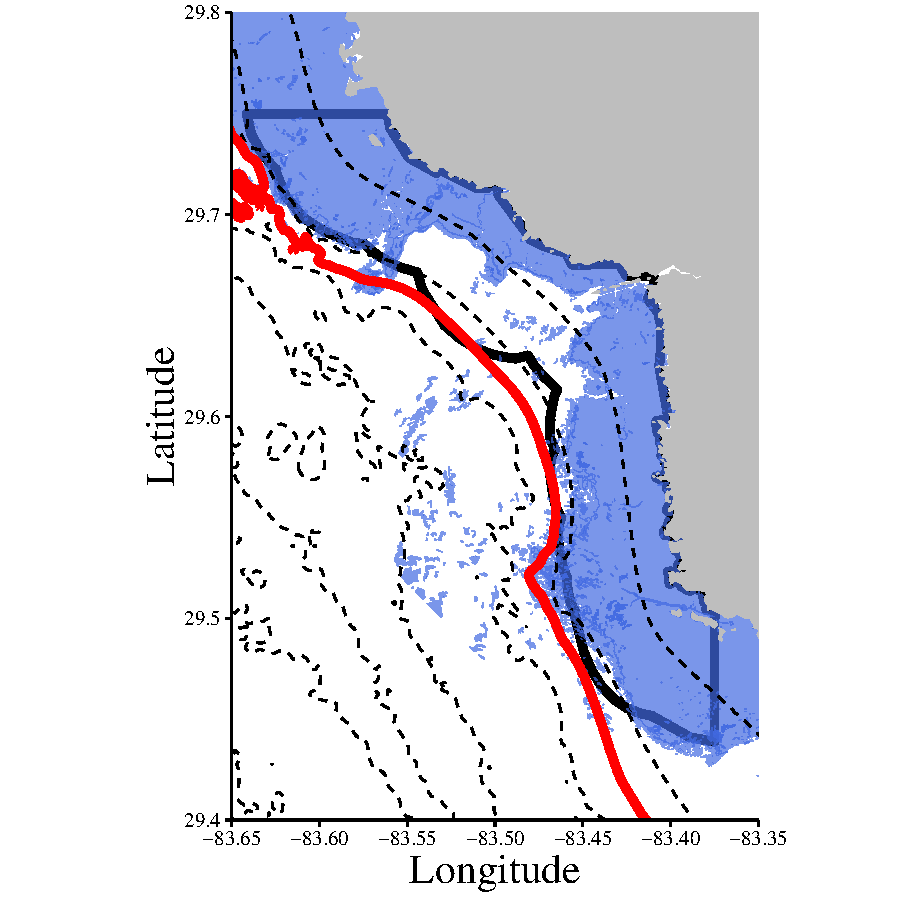
\includegraphics[width=0.5\textwidth,page=1]{figs/buff_ex.pdf}
\label{fig:buff_ex1}
}
\subfloat[][Grid of locations and sample areas for estimates]{
\includegraphics[width=0.5\textwidth,page=2]{figs/buff_ex.pdf}
\label{fig:buff_ex2}
}

\subfloat[][Sampled seagrass data for a test point]{
\includegraphics[width=0.5\textwidth,page=3]{figs/buff_ex.pdf}
\label{fig:buff_ex3}
}
\subfloat{
\includegraphics[width=0.5\textwidth,page=4]{figs/buff_ex.pdf}
}
\caption{Examples of data and grid locations for estimating seagrass depth of colonization for a region of the Big Bend, Florida.  \Cref{fig:buff_ex1} shows the seagrass coverage and depth contours at 2 meter intervals, including the whole segment estimate for depth of colonization. \cref{fig:buff_ex2} shows a grid of sampling locations with sampling radii for estimating \ac{doc} and seagrass depth points derived from bathymetry and seagrass coverage layers.  \cref{fig:buff_ex3} shows an example of sampled seagrass depth points for a test location.  Estimates in \cref{fig:est_ex} were obtained from the test location in \cref{fig:buff_ex3}.}
\label{fig:buff_ex}
\end{figure}

% example of depth of col ests for wbid - big bend 820
\begin{figure}
\centerline{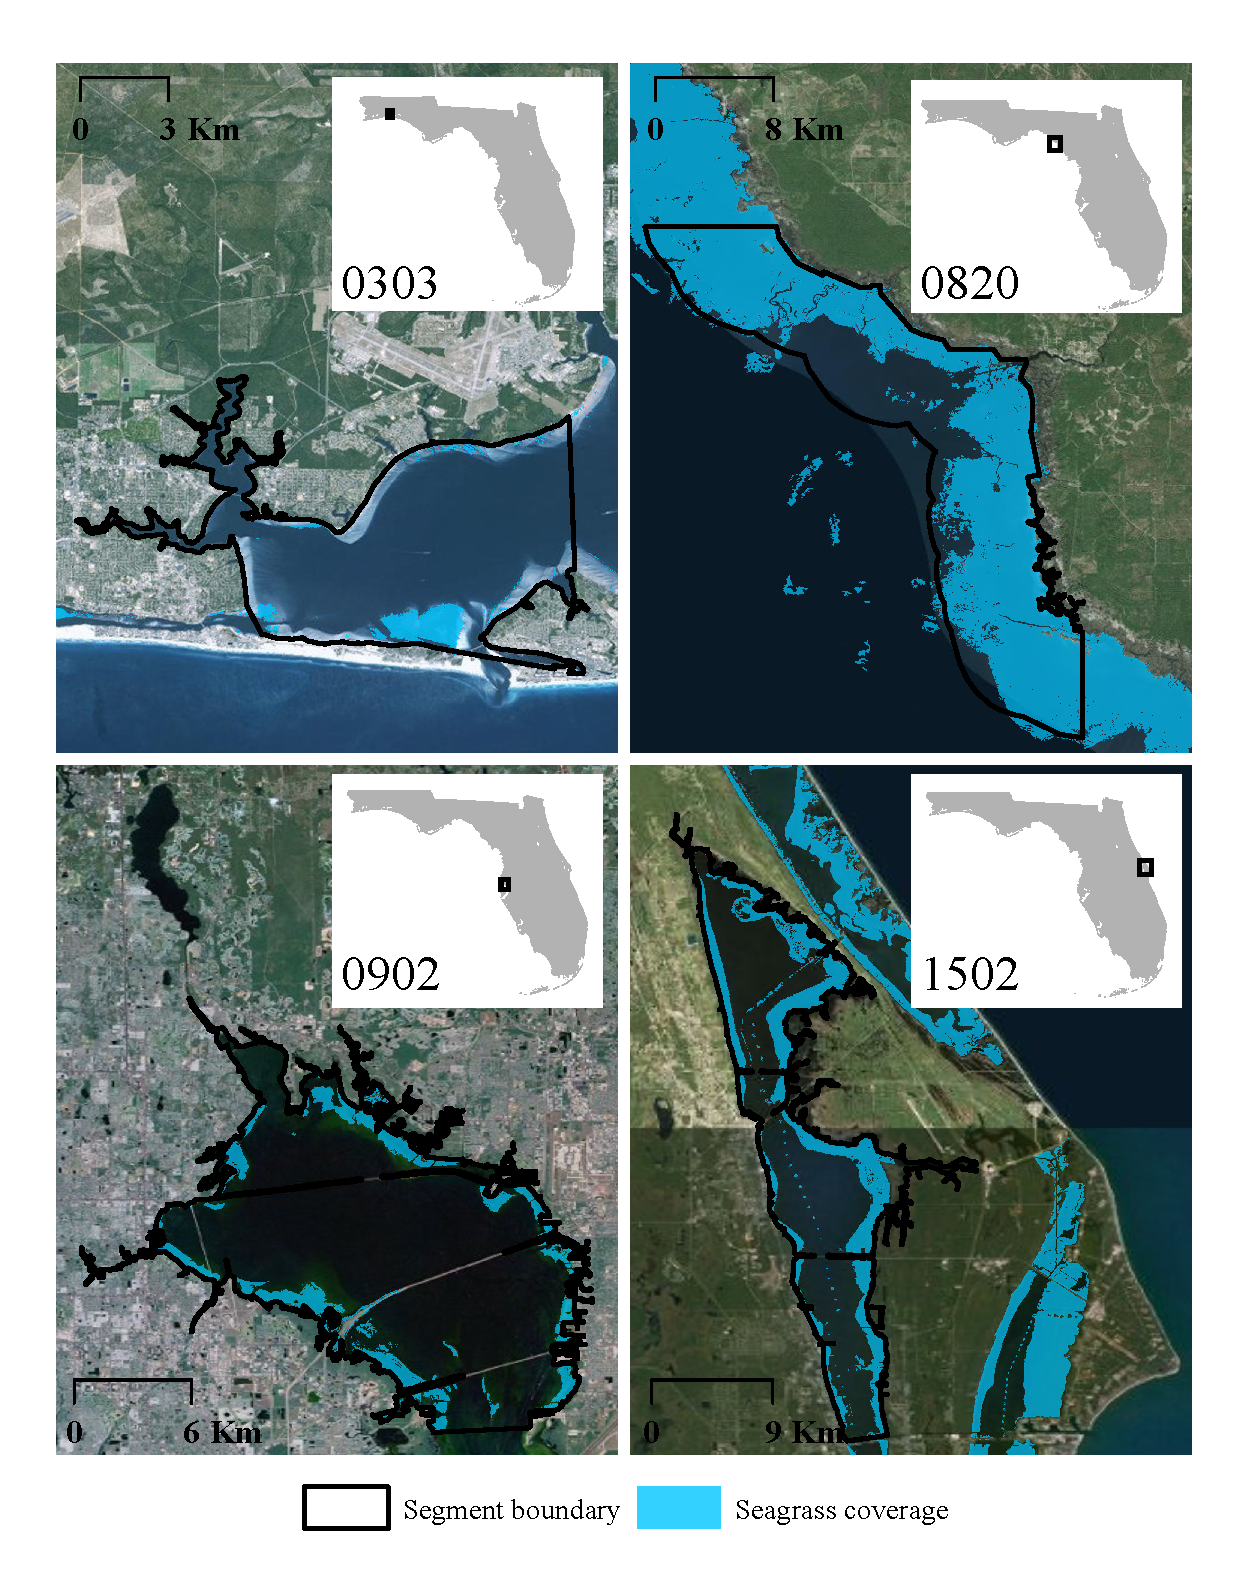
\includegraphics[width = \textwidth]{figs/seg_all.pdf}}
\caption{Locations and seagrass coverage of estuary segments used to evaluate \acl{doc} estimates.  Seagrass coverage layers are from 2006 (BB: Big Bend), 2010 (OTB: Old Tampa Bay), 2009 (UIRL: Upper Indian R. Lagoon), and 2007 (WCB: Western Choctawhatchee Bay).}
\label{fig:seg_all}
\end{figure}

% example of estimating seagrass depth of colonization


% example of depth of col ests for wbid - big bend 820
\begin{figure}
\centering
\subfloat[][Proportion of points with seagrass by depth]{
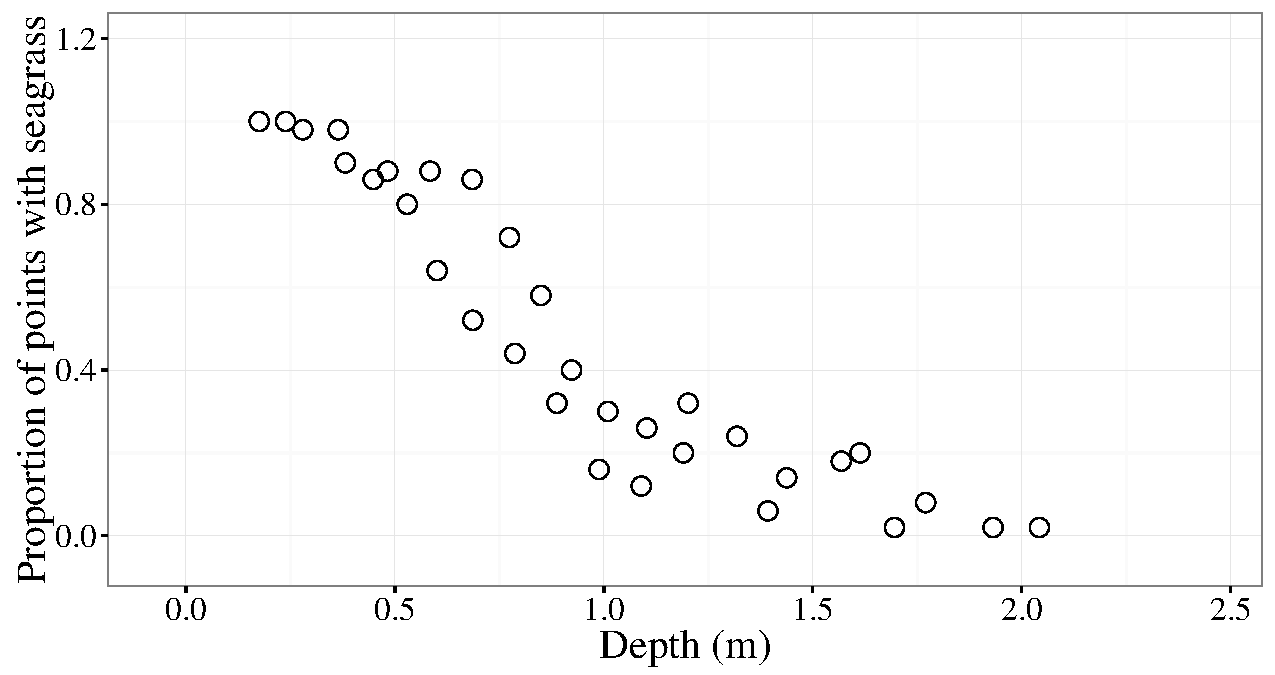
\includegraphics[page=1,width=0.5\textwidth]{figs/est_ex.pdf}
\label{fig:est_ex1}
}

\subfloat[][Logistic growth curve fit through points]{
\includegraphics[page=2,width=0.5\textwidth]{figs/est_ex.pdf}
\label{fig:est_ex2}
}

\subfloat[][Depth estimates]{
\includegraphics[page=3,width=0.5\textwidth]{figs/est_ex.pdf}
\label{fig:est_ex3}
}
\caption{Methods for estimating seagrass depth of colonization using sampled seagrass depth points around a single location. \Cref{fig:est_ex1} is the proportion of points with seagrass by depth using depth points within the buffer of the test location in \cref{fig:buff_ex}.  \Cref{fig:est_ex2} adds a decreasing logistic growth curve fit through the points.  \Cref{fig:est_ex3} shows three depth estimates based on a linear curve through the inflection point of logistic growth curve, including 95\% confidence intervals based on the lighter green area around the linear curve.}
\label{fig:est_ex}
\end{figure}

% grid examples for each segment

\begin{figure}
\centering
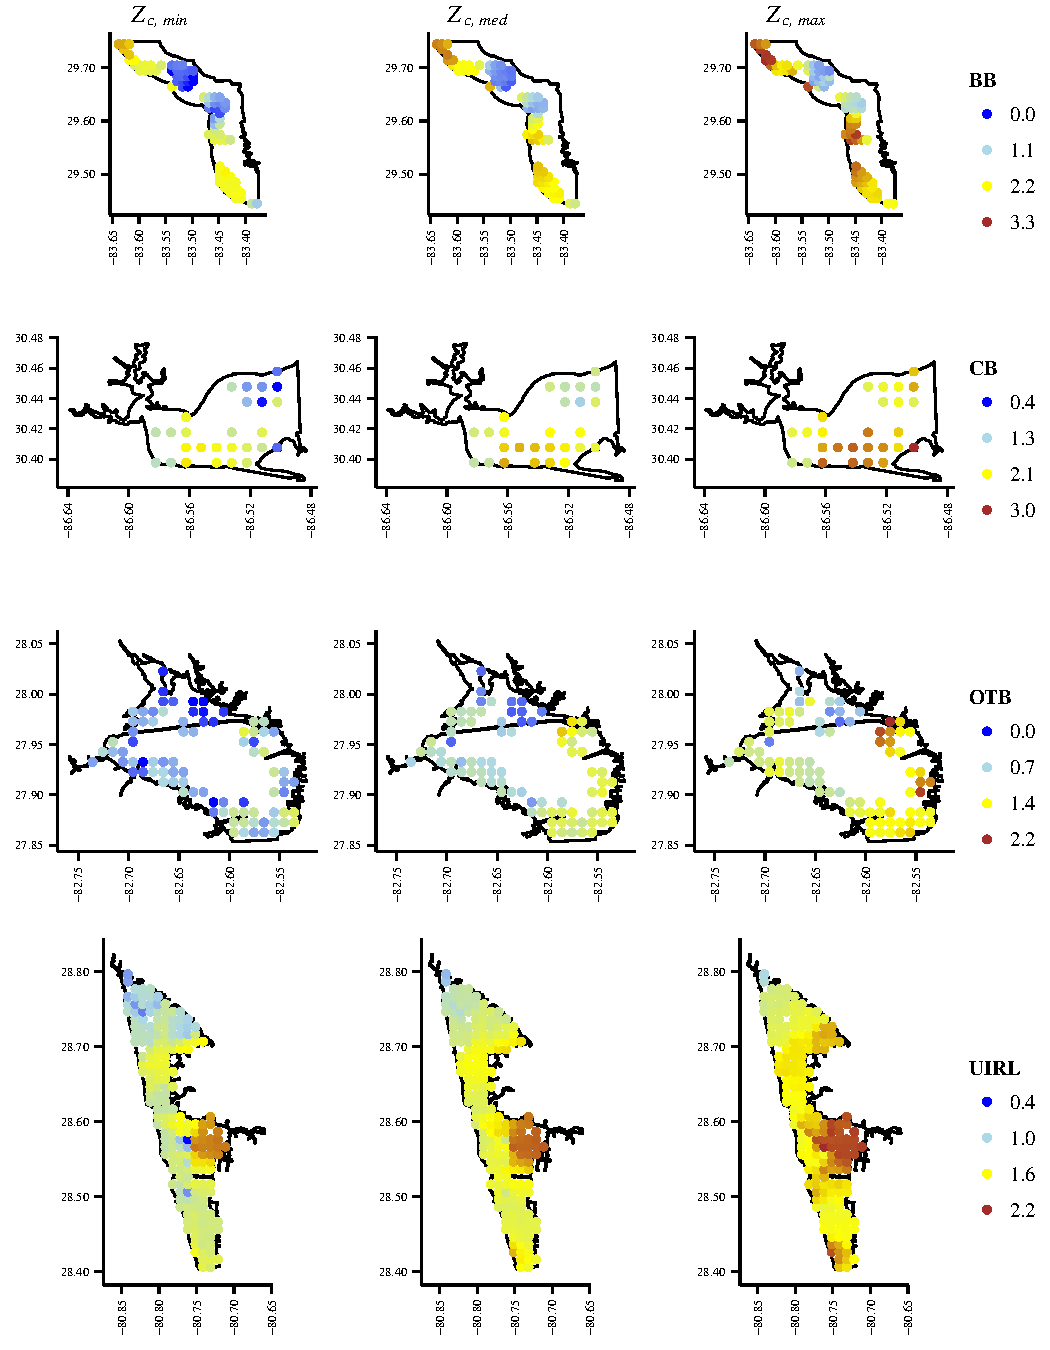
\includegraphics[width = 0.95\textwidth]{figs/all_ests.pdf}
\caption{Spatially-resolved estimates of seagrass depth limits (m) for four coastal segments of Florida. Maximum depth of colonization ($Z_{c,\,max}$) estimates are on the left and correspondings widths of the 95\% confidence intervals are on the right.  Estimates are assigned to grid locations for each segment, where grid spacing was fixed at 0.02 decimal degrees.  Radii for sampling seagrass bathymetric data around each grid location were fixed at 0.06 decimal degrees. From top to bottom: Big Bend, Old Tampa Bay, Upper Indian R. Lagoon, Western Choctawhatchee Bay.}
\label{fig:all_ests}
\end{figure}

% satellite estimates of water clarity for choc bay

\begin{figure}
\centering
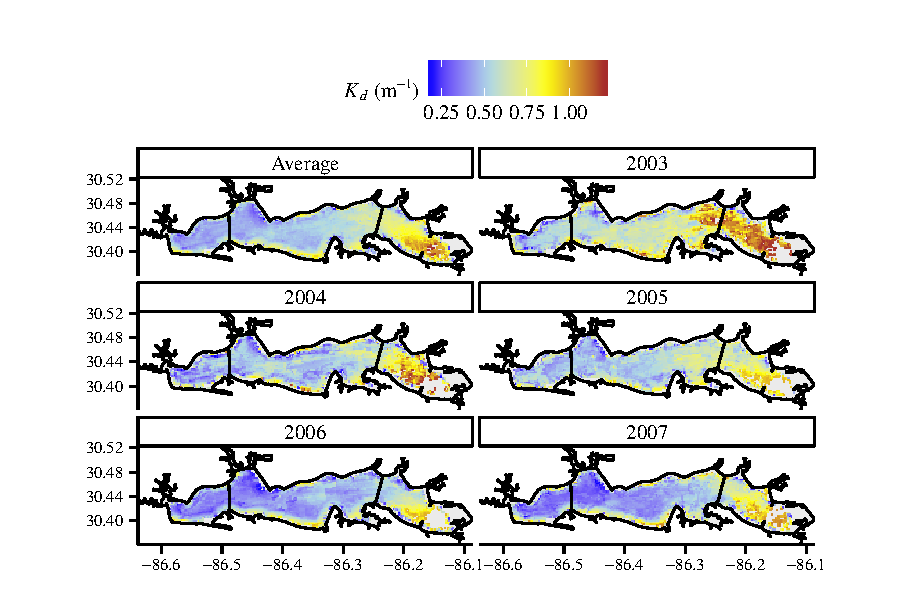
\includegraphics[width = \textwidth]{figs/kd_choc.pdf}
\caption{Satellite estimated light attenuation for Choctawhatchee Bay.  Each facet is an annual average of light attenuation for available years of satellite data up to the year of seagrass coverage used to estimate depth of colonization.  The first facet is an average of all years.  See \cref{fig:light_choc} for segment identification.}
\label{fig:kd_choc}
\end{figure}

% satellite estimates of water clarity for Tampa Bay

\begin{figure}
\centering
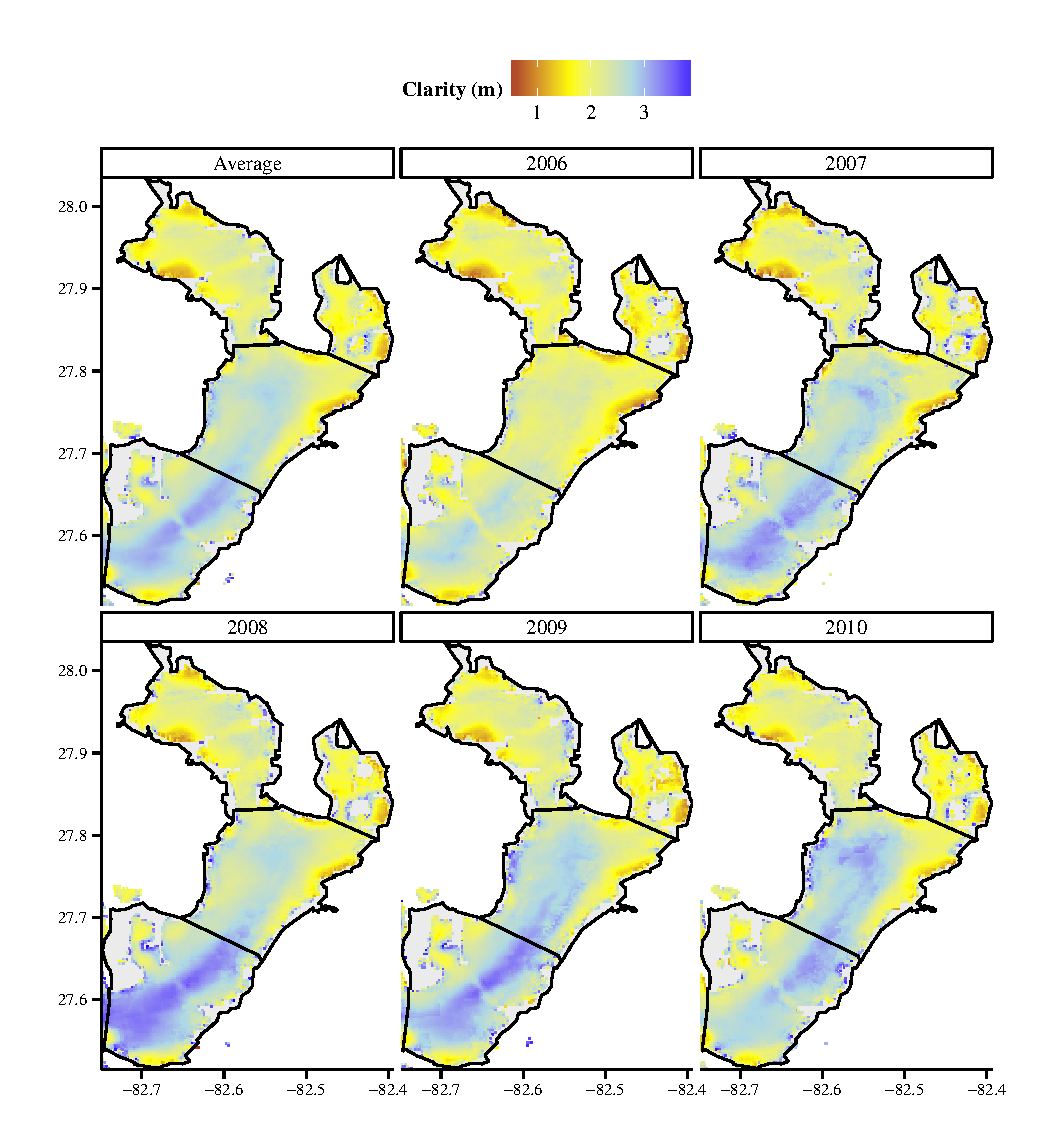
\includegraphics[width = \textwidth]{figs/clarity_tb.pdf}
\caption{Satellite estimated water clarity for Tampa Bay.  Each facet is an annual average of water clarity for available years of satellite data. The first facet is an average of all years.  See \cref{fig:light_tb} for segment identification.}
\label{fig:clarity_tb}
\end{figure}

% estimated light requirements for Choctawhatchee Bay

\begin{figure}
\centering
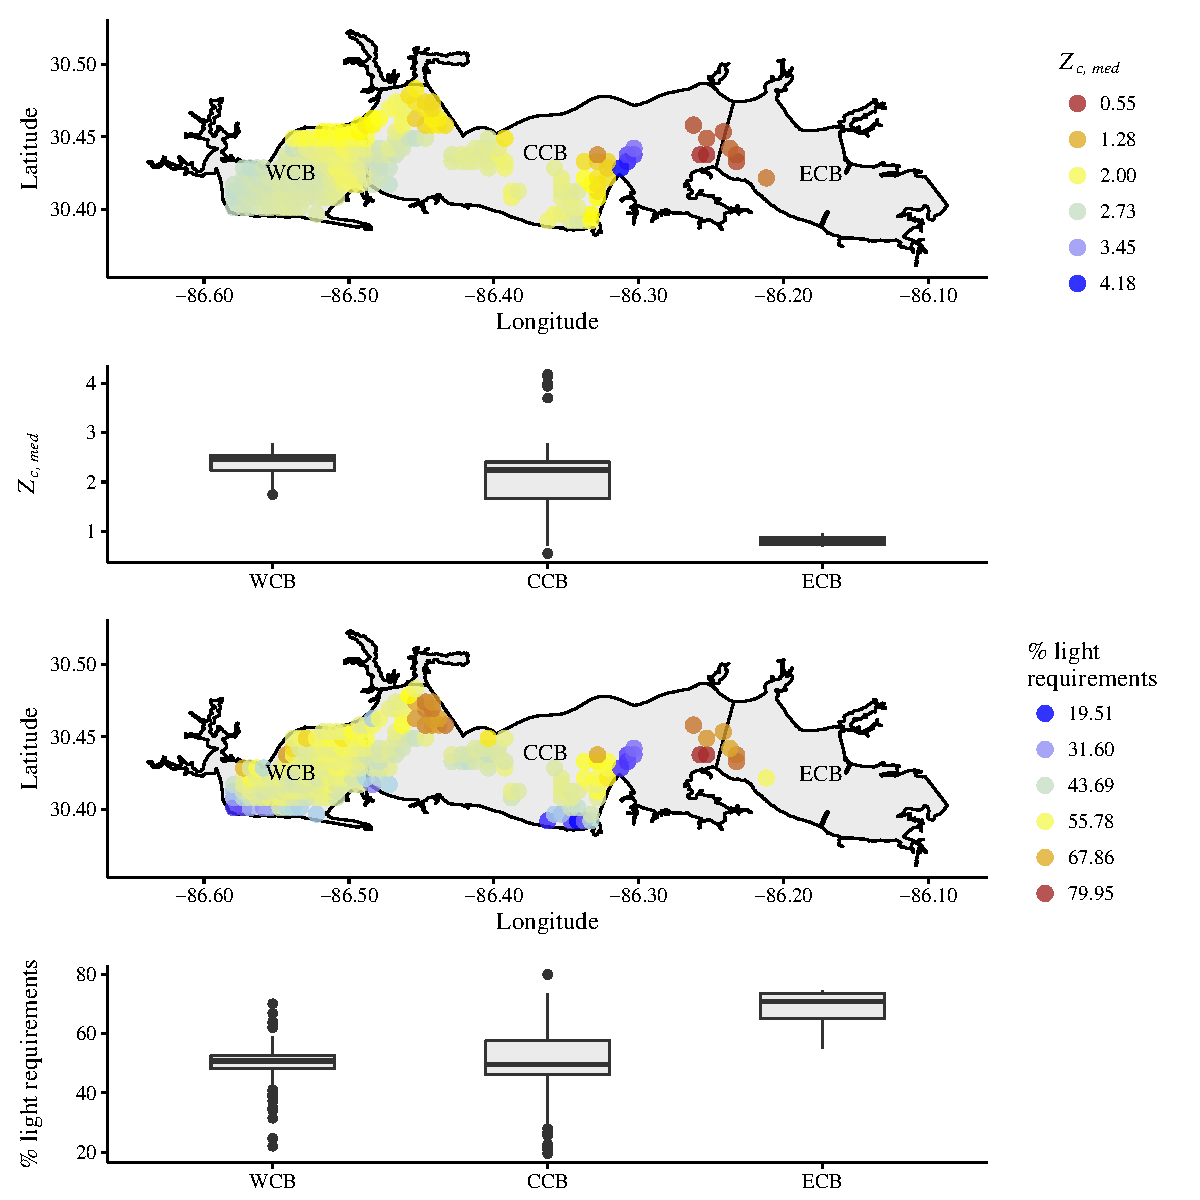
\includegraphics[width = 0.95\textwidth]{figs/light_choc.pdf}
\caption{Estimated maximum depths of seagrass colonization and light requirements for multiple locations in Choctawhatchee Bay, Florida. Locations are those where water clarity estimates were available from satellite observations and seagrass depth of colonization was estimable using a radius of 0.04 decimal degrees.  Estimates are also summarized by bay segment as boxplots where the dimensions are the 25\textsuperscript{th} percentile, median, and 75\textsuperscript{th} percentile.  Whiskers extend beyond the boxes as 1.5 multiplied by the interquartile range. CCB: Central Choctawhatchee Bay, ECB: East Choctawhatchee Bay, WCB: West Choctawhatchee Bay.}
\label{fig:light_choc}
\end{figure}

% estimated light requirements for Tampa Bay

\begin{figure}
\centering
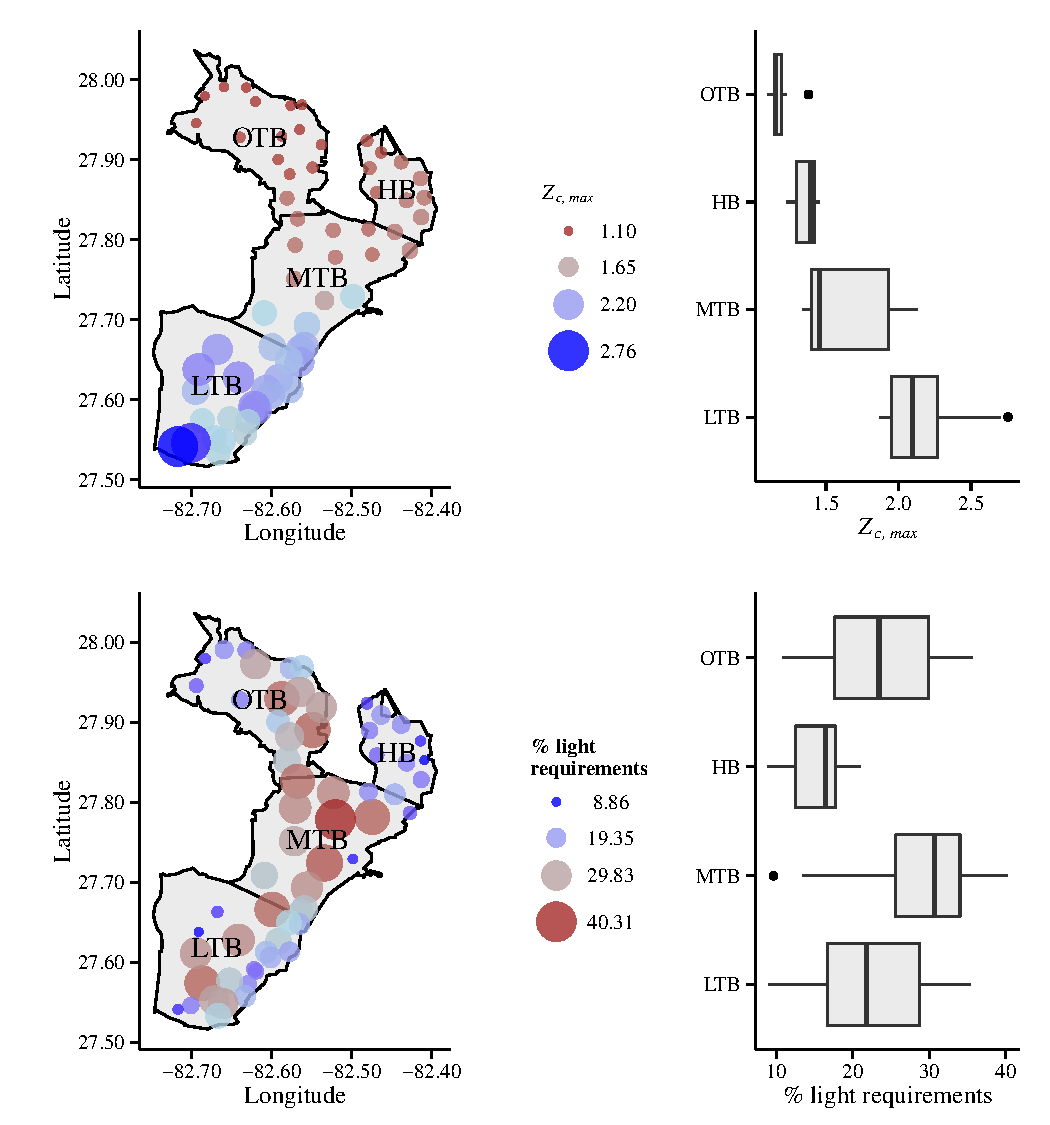
\includegraphics[width = 0.95\textwidth]{figs/light_tb.pdf}
\caption{Estimated maximum depths of seagrass colonization and light requirements for multiple locations in Tampa Bay, Florida. Locations are those where water clarity estimates were available from satellite observations and seagrass depth of colonization was estimable using a radius of 0.1 decimal degrees.  Estimates are also summarized by bay segment as boxplots as in \cref{fig:light_choc}. HB: Hillsborough Bay, LTB: Lower Tampa Bay, MTB: Middle Tampa Bay, OTB: Old Tampa Bay.}
\label{fig:light_tb}
\end{figure}

% estimated light requirements for Indian River Lagoon

\begin{figure}
\centering
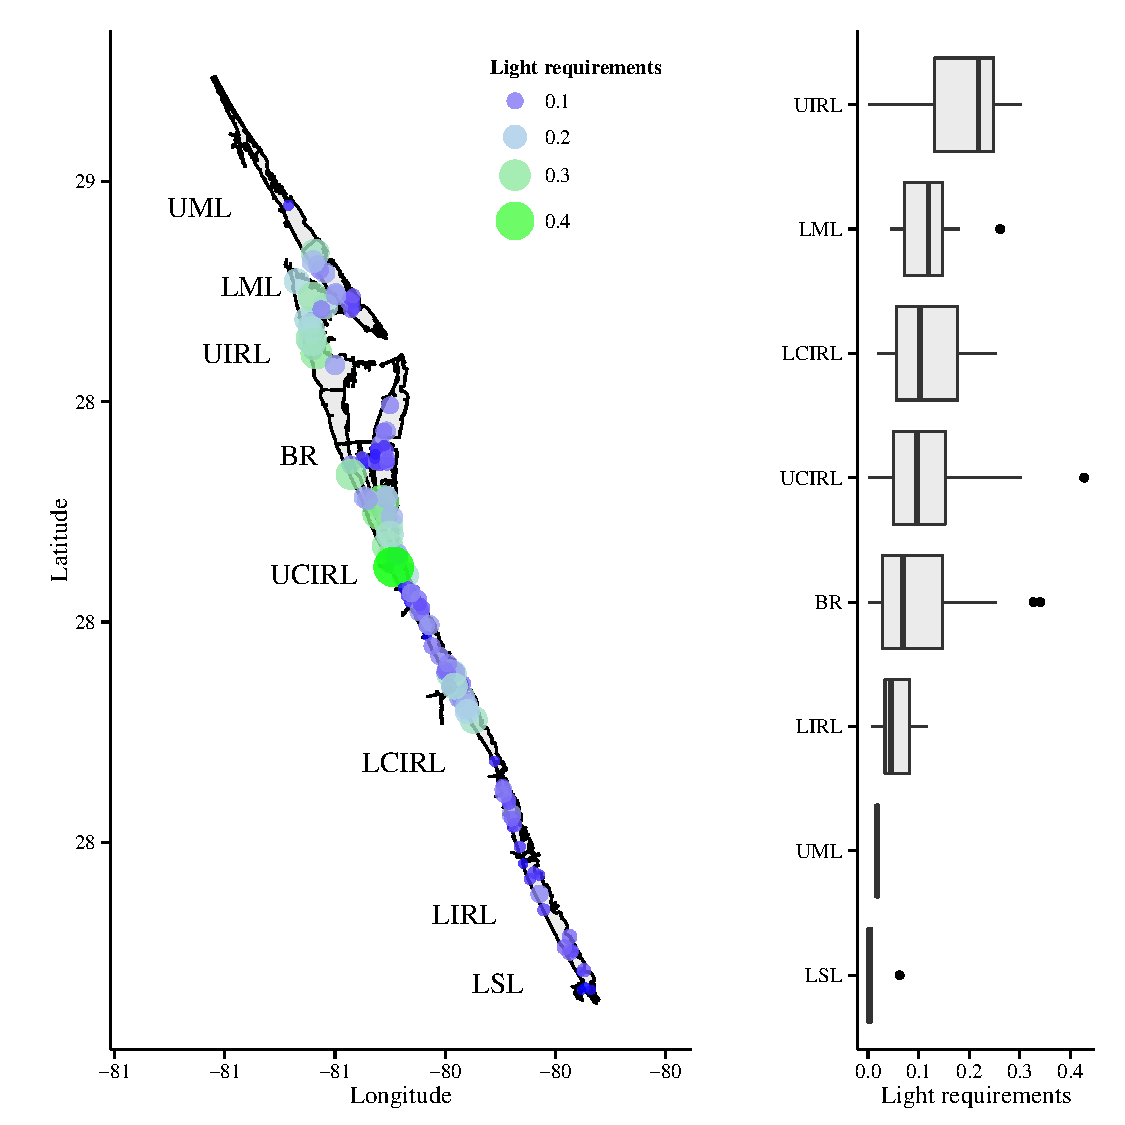
\includegraphics[width = 0.8\textwidth]{figs/light_irl.pdf}
\caption{Estimated maximum depths of seagrass colonization and light requirements for multiple locations in Indian River Lagoon, Florida.  Map locations are georeferenced observations of water clarity in the Florida \acl{IWR} database, update 40.  Estimates are also summarized by bay segment as boxplots as in \cref{fig:light_choc}. Light requirements are based on averaged secchi values within ten years of the seagrass coverage data and estimated maximum depth of colonization using a radius of 0.15 decimal degrees for each secchi location to sample seagrass depth points. BR: Banana R., LCIRL: Lower Central Indian R. Lagoon, LIRL: Lower Indian R. Lagoon, LML: Lower Mosquito Lagoon, LSL: Lower St. Lucie, UCIRL: Upper Central Indian R. Lagoon, UIRL: Upper Indian R. Lagoon, UML: Upper Mosquito Lagoon.}
\label{fig:light_irl}
\end{figure}

\end{document}
